% ============================================================================
% Downhill-Simplex-Algorithmus
% ============================================================================

\ifdefined\outputformat\else\def\outputformat{}\fi
\documentclass[\outputformat]{beamer}

\usetheme[
  pageofpages=von, % String used between the current and the total page count.
  alternativetitlepage=false, % Use the fancy title page.
  titlepagelogo=logo, % Logo for the first page.
]{Torino}

\usepackage[utf8]{inputenc} % Schriftkodierung mit Umlauten
\usepackage[T1]{fontenc}
\usepackage[ngerman]{babel}
\usepackage{graphicx} % Grafiken
\usepackage{tabularx}
\usepackage{booktabs}
\usepackage{textcomp}
\usepackage{amsmath}
\usepackage{pifont}

\usepackage{multirow} 

\usepackage{bm}
\usepackage{bbm}
\usepackage{color}
\usepackage{tikz}
\usetikzlibrary{arrows,shapes,snakes}

\usepackage{colortbl}

\graphicspath{{abbildungen/}}

%\beamersetuncovermixins{\opaqueness<1>{25}}{\opaqueness<2->{15}}
\logo{
\includegraphics[height=0.0625\paperheight]{HSR_Logo_CMYK.pdf}}

\author{Selina Malacarne \and\\ Raphael Nestler}
\title{Simplex Algorithmus für nichtlineare Optimierungsprobleme}
\subtitle{Simplex-Downhill Algorithmus}
%\institute{
\includegraphics[height=0.13\paperheight]{HSR_Logo_CMYK.pdf}}
\date{13. Mai 2013}

\setcounter{tocdepth}{1}

% ============================================================================
\begin{document}

\begin{frame}
\titlepage
\end{frame}

\begin{frame}{Programm}
\tableofcontents
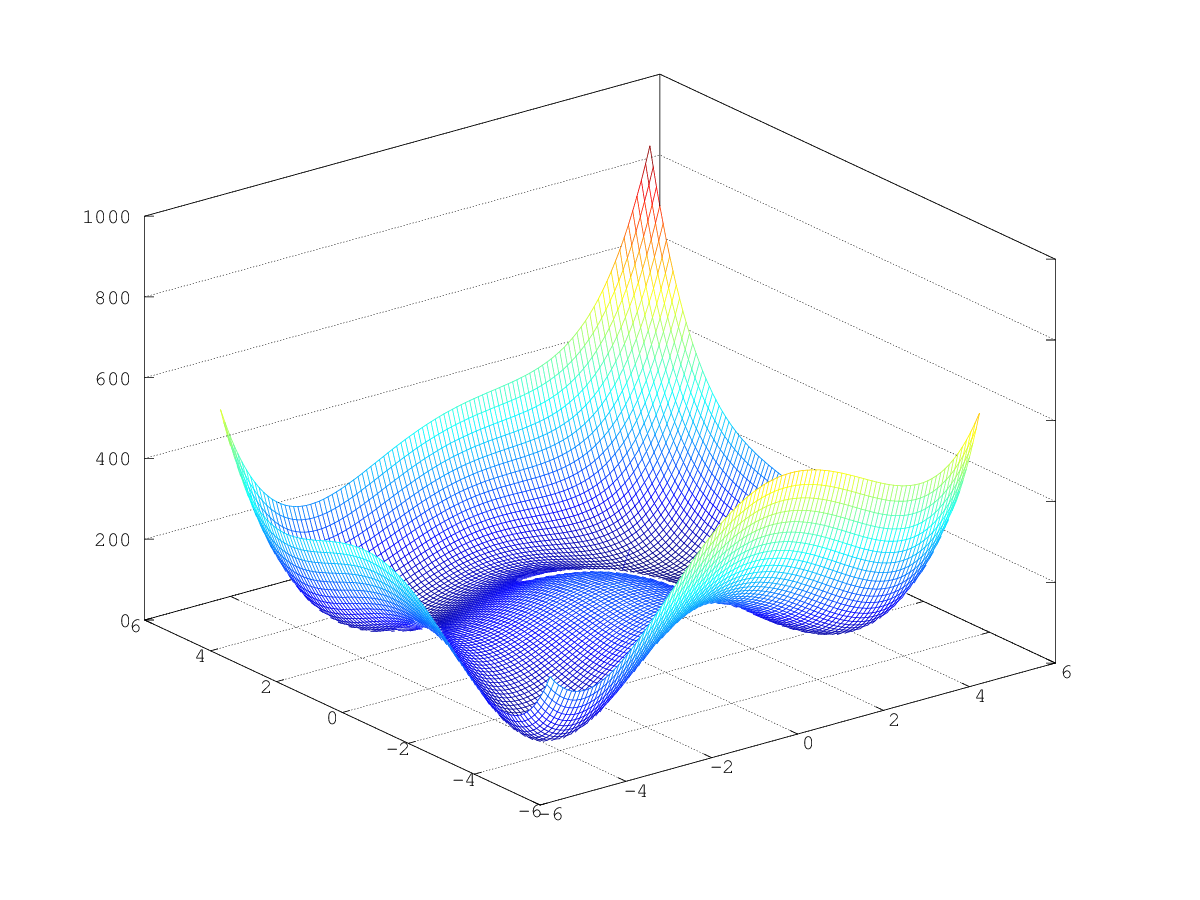
\includegraphics[height=0.5\paperheight]{himmelblau.png}
\end{frame}

% ============================================================================
\section{Einleitung} 
\begin{frame}{Programm}\tableofcontents[currentsection]\end{frame}

\begin{frame}{Einleitung}
	\begin{itemize}
		\pause\item Beschrieben von John Nelder und Roger Mead ($\approx 1965$)
		\pause\item \textbf{NICHT} verwechseln mit Simplex Algorithmus
		\pause\item Anwendung: 
		\begin{itemize}
			\pause\item Optimierung nichtlinearer Funktionen mit mehreren Parametern 
			\pause\item Kurvenfitten (bspw. Messwerte an Kurve angleichen)
		\end{itemize}	
	\end{itemize}
\end{frame}

\begin{frame}{Merkmale}
	\begin{itemize}
		\pause\item Vorteile\\
			\qquad Benötigt \textbf{keine} Ableitungen\\
			\qquad Einfach und robust\\
			\qquad Zielfunktion muss nicht komplett bekannt sein \\
			\qquad (Parameteroptimierung bei komplexen Simulation)
			
	\end{itemize}
	\begin{itemize}
		\pause\item Nachteile\\
			\qquad Langsam (konvergiert linear)\\
			\qquad Kann in lokales Minima fallen\\
	\end{itemize}

	    
\end{frame}

\begin{frame}{Grundlegendes}
	\begin{minipage}[m]{4cm}
		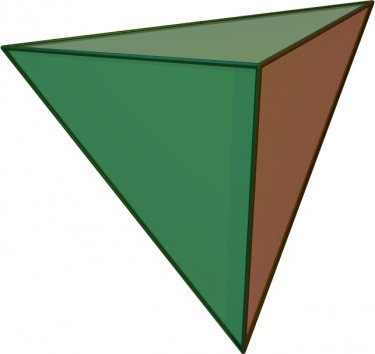
\includegraphics[height=0.3\paperheight]{tetraeder.jpg}
	\end{minipage}
	\begin{minipage}[m]{7cm}
		\begin{itemize}
			\item Anstatt Ableitungen $\rightarrow$ Simplex
			\item Simplex
				\begin{itemize}
					\item m-Eck in n Dimensionen ($m=n+1$)\\
				\end{itemize}
		\end{itemize}
		\begin{tabular}{c|l}
		Dimension & Geometrische Form\\
		\hline
		$n=0$ & Punkt\\
		$n=1$ & Strecke\\
		$n=2$ & Dreieck\\
		$n=3$ & Tetraeder
		\end{tabular} 
		\begin{itemize}
			\pause\item Simplex wird irgendwo in die Zielfunktion gelegt (Testpunkte)
			\pause\item Verhalten an diesen Testpunkten betrachten
			\pause\item Wenn nötig $\rightarrow$ Simplex ändern
		\end{itemize}
	\end{minipage}
\end{frame}

% ============================================================================
\section{Der Algorithmus} 
\begin{frame}{Programm}\tableofcontents[currentsection]\end{frame}

\begin{frame}{Übersicht}
\newcommand{\highlight}{white}

%\usetikzlibrary{arrows}
\begin{tikzpicture}[node distance = 1.7cm,every node/.style={rectangle,fill=white},
  block/.style={draw},
  highlight/.style={draw,fill=\highlight},
  line/.style = {draw,-latex'}
]

\node (start) [block] {N+1 Startpunkte $x_i$ wählen (Simplex bilden)};

\node (a1) [block, below of=start] { $y_i = f(x_i)$ berechnen};

\node (a2) [block, below of=a1] { Bestes ($y_{min}$) und schlechtestes ($y_{max}$) $y_i$ bestimmen};

\node (a3) [block, below of=a2 ]{$y_{min}$ gut genug?};

\node (ende) [block, below of=a3] {Ende};

\node (a4) [highlight, left of=a3, node distance=6cm] {Neuer Simplex bilden};



\path[line] (start) -- (a1);
\path[line] (a1) -> (a2);
\path[line] (a2) -> (a3);

\path[line] (a3) -> node{ja} (ende);
\path[line] (a3) -> node{nein} (a4);

\path[line] (a4)  |-  (a1.west);

\end{tikzpicture}

\end{frame}
\begin{frame}{Übersicht}
\newcommand{\highlight}{green}

%\usetikzlibrary{arrows}
\begin{tikzpicture}[node distance = 1.7cm,every node/.style={rectangle,fill=white},
  block/.style={draw},
  highlight/.style={draw,fill=\highlight},
  line/.style = {draw,-latex'}
]

\node (start) [block] {N+1 Startpunkte $x_i$ wählen (Simplex bilden)};

\node (a1) [block, below of=start] { $y_i = f(x_i)$ berechnen};

\node (a2) [block, below of=a1] { Bestes ($y_{min}$) und schlechtestes ($y_{max}$) $y_i$ bestimmen};

\node (a3) [block, below of=a2 ]{$y_{min}$ gut genug?};

\node (ende) [block, below of=a3] {Ende};

\node (a4) [highlight, left of=a3, node distance=6cm] {Neuer Simplex bilden};



\path[line] (start) -- (a1);
\path[line] (a1) -> (a2);
\path[line] (a2) -> (a3);

\path[line] (a3) -> node{ja} (ende);
\path[line] (a3) -> node{nein} (a4);

\path[line] (a4)  |-  (a1.west);

\end{tikzpicture}

\end{frame}


\begin{frame}{Start}
\begin{columns}[c]
	\column[c]{5cm}{\definecolor{uuuuuu}{rgb}{0.27,0.27,0.27}
\definecolor{zzttqq}{rgb}{0.6,0.2,0}
\definecolor{qqqqff}{rgb}{0,0,1}
\begin{tikzpicture}[line cap=round,line join=round,>=triangle 45,x=1.0cm,y=1.0cm]
\clip(5.32,0.26) rectangle (11.46,4.08);
\fill[color=zzttqq,fill=zzttqq,fill opacity=0.1] (5.74,2.92) -- (10.36,3.74) -- (11,1.52) -- cycle;
\draw [color=zzttqq] (5.74,2.92)-- (10.36,3.74);
\draw [color=zzttqq] (10.36,3.74)-- (11,1.52);
\draw [color=zzttqq] (11,1.52)-- (5.74,2.92);
\draw [color=zzttqq] (11,1.52)-- (5.74,2.92);
\begin{scriptsize}
\fill [color=qqqqff] (5.74,2.92) circle (1.5pt);
\draw[color=qqqqff] (5.75,3.02) node {$x_{min}$};
\fill [color=qqqqff] (10.36,3.74) circle (1.5pt);
\draw[color=qqqqff] (10.51,3.81) node {$x_{max}$};
\fill [color=qqqqff] (11,1.52) circle (1.5pt);
\draw[color=qqqqff] (11.07,1.59) node {$x_3$};
\fill [color=uuuuuu] (9.03,2.73) circle (1.5pt);
\draw[color=uuuuuu] (9.13,2.7) node {$x_m$};
\end{scriptsize}
\end{tikzpicture}
}
	\column{5cm}{
		\begin{itemize}
		\item $x_{min}$: Bester Punkt
		\item $x_{max}$: Schlechtester Punkt
		\item $x_{m}$: Mittelwert
		\end{itemize}
	}
\end{columns}
\end{frame}


\begin{frame}{Neuer Simplex bilden}
Gemäss Vorschlag von Wikipedia\footnote{\url{http://de.wikipedia.org/wiki/Downhill-Simplex-Verfahren}}

Vier mögliche Varianten
\begin{enumerate}
\item Reflexion
\item Expansion
\item Kontraktion 1/2
\item Komprimierung
\end{enumerate}
\end{frame}

\begin{frame}{Auswahl der Variante}
\resizebox{1\textwidth}{!}{
\usetikzlibrary{shapes}
\begin{tikzpicture}[
  top/.style={draw,align=center,text width=5cm},
  med/.style={draw,align=center,text width=5cm},
  fin/.style={ellipse,draw,align=center}
]

\tikzstyle{level 1}=[sibling distance=150mm,align=center]
\tikzstyle{level 2}=[sibling distance=100mm,align=center]
\tikzstyle{level 3}=[sibling distance=80mm]


\node (start) at (0,1.5)[top] {$x_{max}$ am Mittelpunkt des restlichen Simplex ($x_m$) spiegeln $\rightarrow$ $x_{ref}$};

\node[top](top){$y_{ref}$ besser als  $y_{min}$?}
	child { node {Ja} child {child { child  { child { child {
		node[med] {Expansion: In Richtung $y_{ref}$ mit Faktor $\gamma$ Strecken  $\rightarrow y_{streck} $}
		child{
			node[med]  {$y_{streck}$ besser als $y_{min}$?}
			child { node {ja}
			child { node [fin]{$x_{max}$ mit $x_{streck}$ ersetzen} }}
			child { node {nein}
			child { node(a2) [fin]{$x_{max}$ mit $x_{ref}$ ersetzen} }}
		}
	}}}}}}
	child {
		node {Nein}
		child  {
		node [med] {$y_{ref}$ besser als zweitschlechtestes $y_i$ ?}
		child { node (b1) [] {Ja} }
		child { node {Nein} 
		child { node[med] {Ist $y_{ref}$ besser als $y_{max}$? }
			child {node{Nein}
				child { node (kont)[med] {Kontraktion: Rücke mit Faktor $\beta$ näher an Mittelpunkt $\rightarrow y_{kon}$ }
					child { node[med]  {Ist $y_{kon}$ besser als $y_{max}$?}
						child {node {Ja}
							child {node[fin] {Ersetze $x_{max}$ durch $x_{kon}$}}
						}
						child {node {Nein}
							child {node[fin] {Komprimierung: Rücke alle $x_i$ zu $x_{min}$ } }
						}
					}
				}
			}
			child {node {Ja}
				child { node (zukont)[med] {Ersetze $x_{max}$ durch $x_{ref}$ } }
			}
		}
		}
	}
	}
;
\draw (zukont) -- (kont);
\draw (b1) -- (a2);
\draw (start) --(top);

\end{tikzpicture}
}

\end{frame}
\begin{frame}{Auswahl der Variante}
\newcommand{\highlightref}{green}
\resizebox{1\textwidth}{!}{
\usetikzlibrary{shapes}
\begin{tikzpicture}[
  top/.style={draw,align=center,text width=5cm},
  med/.style={draw,align=center,text width=5cm},
  fin/.style={ellipse,draw,align=center}
]

\tikzstyle{level 1}=[sibling distance=150mm,align=center]
\tikzstyle{level 2}=[sibling distance=100mm,align=center]
\tikzstyle{level 3}=[sibling distance=80mm]


\node (start) at (0,1.5)[top] {$x_{max}$ am Mittelpunkt des restlichen Simplex ($x_m$) spiegeln $\rightarrow$ $x_{ref}$};

\node[top](top){$y_{ref}$ besser als  $y_{min}$?}
	child { node {Ja} child {child { child  { child { child {
		node[med] {Expansion: In Richtung $y_{ref}$ mit Faktor $\gamma$ Strecken  $\rightarrow y_{streck} $}
		child{
			node[med]  {$y_{streck}$ besser als $y_{min}$?}
			child { node {ja}
			child { node [fin]{$x_{max}$ mit $x_{streck}$ ersetzen} }}
			child { node {nein}
			child { node(a2) [fin]{$x_{max}$ mit $x_{ref}$ ersetzen} }}
		}
	}}}}}}
	child {
		node {Nein}
		child  {
		node [med] {$y_{ref}$ besser als zweitschlechtestes $y_i$ ?}
		child { node (b1) [] {Ja} }
		child { node {Nein} 
		child { node[med] {Ist $y_{ref}$ besser als $y_{max}$? }
			child {node{Nein}
				child { node (kont)[med] {Kontraktion: Rücke mit Faktor $\beta$ näher an Mittelpunkt $\rightarrow y_{kon}$ }
					child { node[med]  {Ist $y_{kon}$ besser als $y_{max}$?}
						child {node {Ja}
							child {node[fin] {Ersetze $x_{max}$ durch $x_{kon}$}}
						}
						child {node {Nein}
							child {node[fin] {Komprimierung: Rücke alle $x_i$ zu $x_{min}$ } }
						}
					}
				}
			}
			child {node {Ja}
				child { node (zukont)[med] {Ersetze $x_{max}$ durch $x_{ref}$ } }
			}
		}
		}
	}
	}
;
\draw (zukont) -- (kont);
\draw (b1) -- (a2);
\draw (start) --(top);

\end{tikzpicture}
}

\end{frame}

\begin{frame}{Reflexion}
\begin{columns}[c]
	\column[c]{5cm}{\definecolor{uuuuuu}{rgb}{0.27,0.27,0.27}
\definecolor{zzttqq}{rgb}{0.6,0.2,0}
\definecolor{qqqqff}{rgb}{0,0,1}
\begin{tikzpicture}[line cap=round,line join=round,>=triangle 45,x=1.0cm,y=1.0cm]
\clip(5.32,0.26) rectangle (11.46,4.08);
\fill[color=zzttqq,fill=zzttqq,fill opacity=0.1] (5.74,2.92) -- (10.36,3.74) -- (11,1.52) -- cycle;
\fill[color=zzttqq,fill=zzttqq,fill opacity=0.1] (5.74,2.92) -- (7.71,1.71) -- (11,1.52) -- cycle;
\draw [color=zzttqq] (5.74,2.92)-- (10.36,3.74);
\draw [color=zzttqq] (10.36,3.74)-- (11,1.52);
\draw [color=zzttqq] (11,1.52)-- (5.74,2.92);
\draw (9.03,2.73)-- (7.71,1.71);
\draw [color=zzttqq] (5.74,2.92)-- (7.71,1.71);
\draw [color=zzttqq] (7.71,1.71)-- (11,1.52);
\draw [color=zzttqq] (11,1.52)-- (5.74,2.92);
\draw [color=zzttqq] (11,1.52)-- (5.74,2.92);
\begin{scriptsize}
\fill [color=qqqqff] (5.74,2.92) circle (1.5pt);
\draw[color=qqqqff] (5.75,3.02) node {$x_{min}$};
\fill [color=qqqqff] (10.36,3.74) circle (1.5pt);
\draw[color=qqqqff] (10.51,3.81) node {$x_{max}$};
\fill [color=qqqqff] (11,1.52) circle (1.5pt);
\draw[color=qqqqff] (11.07,1.59) node {$x_3$};
\fill [color=uuuuuu] (9.03,2.73) circle (1.5pt);
\draw[color=uuuuuu] (9.13,2.7) node {$x_m$};
\fill [color=qqqqff] (7.71,1.71) circle (1.5pt);
\draw[color=qqqqff] (7.91,1.67) node {$x_{ref}$};
\end{scriptsize}
\end{tikzpicture}
}
	\column{5cm}{$x_{ref} = x_m + \alpha(x_m-x_{max})$
	
	\pause In welche Richtung wird es besser? Approximation mit Ebene.
	
	\pause $\alpha$ typischerweise 2
	
	\pause In der Literatur wird $x_m$ oft ohne $x_{max}$ gebildet dafür ein $\alpha$ von 1 verwendet
	}
\end{columns}
\end{frame}

\begin{frame}{Auswahl der Variante}
\newcommand{\highlightexp}{green}
\resizebox{1\textwidth}{!}{
\usetikzlibrary{shapes}
\begin{tikzpicture}[
  top/.style={draw,align=center,text width=5cm},
  med/.style={draw,align=center,text width=5cm},
  fin/.style={ellipse,draw,align=center}
]

\tikzstyle{level 1}=[sibling distance=150mm,align=center]
\tikzstyle{level 2}=[sibling distance=100mm,align=center]
\tikzstyle{level 3}=[sibling distance=80mm]


\node (start) at (0,1.5)[top] {$x_{max}$ am Mittelpunkt des restlichen Simplex ($x_m$) spiegeln $\rightarrow$ $x_{ref}$};

\node[top](top){$y_{ref}$ besser als  $y_{min}$?}
	child { node {Ja} child {child { child  { child { child {
		node[med] {Expansion: In Richtung $y_{ref}$ mit Faktor $\gamma$ Strecken  $\rightarrow y_{streck} $}
		child{
			node[med]  {$y_{streck}$ besser als $y_{min}$?}
			child { node {ja}
			child { node [fin]{$x_{max}$ mit $x_{streck}$ ersetzen} }}
			child { node {nein}
			child { node(a2) [fin]{$x_{max}$ mit $x_{ref}$ ersetzen} }}
		}
	}}}}}}
	child {
		node {Nein}
		child  {
		node [med] {$y_{ref}$ besser als zweitschlechtestes $y_i$ ?}
		child { node (b1) [] {Ja} }
		child { node {Nein} 
		child { node[med] {Ist $y_{ref}$ besser als $y_{max}$? }
			child {node{Nein}
				child { node (kont)[med] {Kontraktion: Rücke mit Faktor $\beta$ näher an Mittelpunkt $\rightarrow y_{kon}$ }
					child { node[med]  {Ist $y_{kon}$ besser als $y_{max}$?}
						child {node {Ja}
							child {node[fin] {Ersetze $x_{max}$ durch $x_{kon}$}}
						}
						child {node {Nein}
							child {node[fin] {Komprimierung: Rücke alle $x_i$ zu $x_{min}$ } }
						}
					}
				}
			}
			child {node {Ja}
				child { node (zukont)[med] {Ersetze $x_{max}$ durch $x_{ref}$ } }
			}
		}
		}
	}
	}
;
\draw (zukont) -- (kont);
\draw (b1) -- (a2);
\draw (start) --(top);

\end{tikzpicture}
}

\end{frame}

\begin{frame}{Expansion}
\begin{columns}[c]
	\column[c]{5cm}{\resizebox{1\textwidth}{!}{
\definecolor{uuuuuu}{rgb}{0.27,0.27,0.27}
\definecolor{zzttqq}{rgb}{0.6,0.2,0}
\definecolor{qqqqff}{rgb}{0,0,1}
\begin{tikzpicture}[line cap=round,line join=round,>=triangle 45,x=1.0cm,y=1.0cm]
\clip(4.51,0.05) rectangle (11.48,4.25);
\fill[color=zzttqq,fill=zzttqq,fill opacity=0.1] (5.74,3) -- (10.36,4) -- (11,2) -- cycle;
\fill[color=zzttqq,fill=zzttqq,fill opacity=0.1] (5.74,3) -- (6.38,1) -- (11,2) -- cycle;
\fill[color=zzttqq,fill=zzttqq,fill opacity=0.1] (5.74,3) -- (5.39,0.25) -- (11,2) -- cycle;
\draw [color=zzttqq] (5.74,3)-- (10.36,4);
\draw [color=zzttqq] (10.36,4)-- (11,2);
\draw [color=zzttqq] (11,2)-- (5.74,3);
\draw (8.37,2.5)-- (6.38,1);
\draw (8.37,2.5)-- (5.39,0.25);
\draw [color=zzttqq] (5.74,3)-- (6.38,1);
\draw [color=zzttqq] (6.38,1)-- (11,2);
\draw [color=zzttqq] (11,2)-- (5.74,3);
\draw [color=zzttqq] (5.74,3)-- (5.39,0.25);
\draw [color=zzttqq] (5.39,0.25)-- (11,2);
\draw [color=zzttqq] (11,2)-- (5.74,3);
\begin{scriptsize}
\fill [color=qqqqff] (5.74,3) circle (1.5pt);
\draw[color=qqqqff] (5.75,3.11) node {$x_{min}$};
\fill [color=qqqqff] (10.36,4) circle (1.5pt);
\draw[color=qqqqff] (10.53,4.07) node {$x_{max}$};
\fill [color=qqqqff] (11,2) circle (1.5pt);
\draw[color=qqqqff] (11.08,2.08) node {$x_3$};
\fill [color=uuuuuu] (8.37,2.5) circle (1.5pt);
\draw[color=uuuuuu] (8.48,2.47) node {$x_m$};
\fill [color=qqqqff] (6.38,1) circle (1.5pt);
\draw[color=qqqqff] (6.62,0.95) node {$x_{ref}$};
\fill [color=uuuuuu] (5.39,0.25) circle (1.5pt);
\draw[color=uuuuuu] (5.6,0.19) node {$x_{streck}$};
\end{scriptsize}
\end{tikzpicture}
}
}
	\column{5cm}{$x_{streck} = x_{ref} + \gamma (x_{ref} - x_m)$
	
	\pause What if we try more?
	
	\pause $\gamma$ typischerweise 2.67
		
	\pause Verhält sich aufgrund unser Variante von $x_m$ ein wenig anders
	}
\end{columns}
\end{frame}

\begin{frame}{Auswahl der Variante}
\newcommand{\highlightrefb}{green}
\resizebox{1\textwidth}{!}{
\usetikzlibrary{shapes}
\begin{tikzpicture}[
  top/.style={draw,align=center,text width=5cm},
  med/.style={draw,align=center,text width=5cm},
  fin/.style={ellipse,draw,align=center}
]

\tikzstyle{level 1}=[sibling distance=150mm,align=center]
\tikzstyle{level 2}=[sibling distance=100mm,align=center]
\tikzstyle{level 3}=[sibling distance=80mm]


\node (start) at (0,1.5)[top] {$x_{max}$ am Mittelpunkt des restlichen Simplex ($x_m$) spiegeln $\rightarrow$ $x_{ref}$};

\node[top](top){$y_{ref}$ besser als  $y_{min}$?}
	child { node {Ja} child {child { child  { child { child {
		node[med] {Expansion: In Richtung $y_{ref}$ mit Faktor $\gamma$ Strecken  $\rightarrow y_{streck} $}
		child{
			node[med]  {$y_{streck}$ besser als $y_{min}$?}
			child { node {ja}
			child { node [fin]{$x_{max}$ mit $x_{streck}$ ersetzen} }}
			child { node {nein}
			child { node(a2) [fin]{$x_{max}$ mit $x_{ref}$ ersetzen} }}
		}
	}}}}}}
	child {
		node {Nein}
		child  {
		node [med] {$y_{ref}$ besser als zweitschlechtestes $y_i$ ?}
		child { node (b1) [] {Ja} }
		child { node {Nein} 
		child { node[med] {Ist $y_{ref}$ besser als $y_{max}$? }
			child {node{Nein}
				child { node (kont)[med] {Kontraktion: Rücke mit Faktor $\beta$ näher an Mittelpunkt $\rightarrow y_{kon}$ }
					child { node[med]  {Ist $y_{kon}$ besser als $y_{max}$?}
						child {node {Ja}
							child {node[fin] {Ersetze $x_{max}$ durch $x_{kon}$}}
						}
						child {node {Nein}
							child {node[fin] {Komprimierung: Rücke alle $x_i$ zu $x_{min}$ } }
						}
					}
				}
			}
			child {node {Ja}
				child { node (zukont)[med] {Ersetze $x_{max}$ durch $x_{ref}$ } }
			}
		}
		}
	}
	}
;
\draw (zukont) -- (kont);
\draw (b1) -- (a2);
\draw (start) --(top);

\end{tikzpicture}
}

\end{frame}

\begin{frame}{Auswahl der Variante}
\newcommand{\highlightcona}{green}
\resizebox{1\textwidth}{!}{
\usetikzlibrary{shapes}
\begin{tikzpicture}[
  top/.style={draw,align=center,text width=5cm},
  med/.style={draw,align=center,text width=5cm},
  fin/.style={ellipse,draw,align=center}
]

\tikzstyle{level 1}=[sibling distance=150mm,align=center]
\tikzstyle{level 2}=[sibling distance=100mm,align=center]
\tikzstyle{level 3}=[sibling distance=80mm]


\node (start) at (0,1.5)[top] {$x_{max}$ am Mittelpunkt des restlichen Simplex ($x_m$) spiegeln $\rightarrow$ $x_{ref}$};

\node[top](top){$y_{ref}$ besser als  $y_{min}$?}
	child { node {Ja} child {child { child  { child { child {
		node[med] {Expansion: In Richtung $y_{ref}$ mit Faktor $\gamma$ Strecken  $\rightarrow y_{streck} $}
		child{
			node[med]  {$y_{streck}$ besser als $y_{min}$?}
			child { node {ja}
			child { node [fin]{$x_{max}$ mit $x_{streck}$ ersetzen} }}
			child { node {nein}
			child { node(a2) [fin]{$x_{max}$ mit $x_{ref}$ ersetzen} }}
		}
	}}}}}}
	child {
		node {Nein}
		child  {
		node [med] {$y_{ref}$ besser als zweitschlechtestes $y_i$ ?}
		child { node (b1) [] {Ja} }
		child { node {Nein} 
		child { node[med] {Ist $y_{ref}$ besser als $y_{max}$? }
			child {node{Nein}
				child { node (kont)[med] {Kontraktion: Rücke mit Faktor $\beta$ näher an Mittelpunkt $\rightarrow y_{kon}$ }
					child { node[med]  {Ist $y_{kon}$ besser als $y_{max}$?}
						child {node {Ja}
							child {node[fin] {Ersetze $x_{max}$ durch $x_{kon}$}}
						}
						child {node {Nein}
							child {node[fin] {Komprimierung: Rücke alle $x_i$ zu $x_{min}$ } }
						}
					}
				}
			}
			child {node {Ja}
				child { node (zukont)[med] {Ersetze $x_{max}$ durch $x_{ref}$ } }
			}
		}
		}
	}
	}
;
\draw (zukont) -- (kont);
\draw (b1) -- (a2);
\draw (start) --(top);

\end{tikzpicture}
}

\end{frame}
\begin{frame}{Kontraktion 1}
\begin{columns}[c]
	\column[c]{5cm}{\resizebox{1\textwidth}{!}{
\definecolor{uuuuuu}{rgb}{0.27,0.27,0.27}
\definecolor{zzttqq}{rgb}{0.6,0.2,0}
\definecolor{qqqqff}{rgb}{0,0,1}
\begin{tikzpicture}[line cap=round,line join=round,>=triangle 45,x=1.0cm,y=1.0cm]
\clip(4.51,0.05) rectangle (11.48,4.25);
\fill[color=zzttqq,fill=zzttqq,fill opacity=0.1] (5.74,3) -- (10.36,4) -- (11,2) -- cycle;
\fill[color=zzttqq,fill=zzttqq,fill opacity=0.1] (5.74,3) -- (9.37,3.25) -- (11,2) -- cycle;
\draw [color=zzttqq] (5.74,3)-- (10.36,4);
\draw [color=zzttqq] (10.36,4)-- (11,2);
\draw [color=zzttqq] (11,2)-- (5.74,3);
\draw [color=zzttqq] (11,2)-- (5.74,3);
\draw [color=zzttqq] (5.74,3)-- (9.37,3.25);
\draw [color=zzttqq] (9.37,3.25)-- (11,2);
\draw [color=zzttqq] (11,2)-- (5.74,3);
\begin{scriptsize}
\fill [color=qqqqff] (5.74,3) circle (1.5pt);
\draw[color=qqqqff] (5.75,3.11) node {$x_{min}$};
\fill [color=qqqqff] (10.36,4) circle (1.5pt);
\draw[color=qqqqff] (10.53,4.07) node {$x_{max}$};
\fill [color=qqqqff] (11,2) circle (1.5pt);
\draw[color=qqqqff] (11.08,2.08) node {$x_3$};
\fill [color=uuuuuu] (8.37,2.5) circle (1.5pt);
\draw[color=uuuuuu] (8.48,2.47) node {$x_m$};
\fill [color=uuuuuu] (9.37,3.25) circle (1.5pt);
\draw[color=uuuuuu] (9.59,3.3) node {$x_{kon}$};
\end{scriptsize}
\end{tikzpicture}
}
}
	\column{5cm}{$x_{con_1}=x_m - \beta (x_m-x_{max})$
	
	\pause Verhält sich aufgrund unser Variante von $x_m$ ein wenig anders
	}
\end{columns}
\end{frame}

\begin{frame}{Auswahl der Variante}
\newcommand{\highlightconb}{green}
\resizebox{1\textwidth}{!}{
\usetikzlibrary{shapes}
\begin{tikzpicture}[
  top/.style={draw,align=center,text width=5cm},
  med/.style={draw,align=center,text width=5cm},
  fin/.style={ellipse,draw,align=center}
]

\tikzstyle{level 1}=[sibling distance=150mm,align=center]
\tikzstyle{level 2}=[sibling distance=100mm,align=center]
\tikzstyle{level 3}=[sibling distance=80mm]


\node (start) at (0,1.5)[top] {$x_{max}$ am Mittelpunkt des restlichen Simplex ($x_m$) spiegeln $\rightarrow$ $x_{ref}$};

\node[top](top){$y_{ref}$ besser als  $y_{min}$?}
	child { node {Ja} child {child { child  { child { child {
		node[med] {Expansion: In Richtung $y_{ref}$ mit Faktor $\gamma$ Strecken  $\rightarrow y_{streck} $}
		child{
			node[med]  {$y_{streck}$ besser als $y_{min}$?}
			child { node {ja}
			child { node [fin]{$x_{max}$ mit $x_{streck}$ ersetzen} }}
			child { node {nein}
			child { node(a2) [fin]{$x_{max}$ mit $x_{ref}$ ersetzen} }}
		}
	}}}}}}
	child {
		node {Nein}
		child  {
		node [med] {$y_{ref}$ besser als zweitschlechtestes $y_i$ ?}
		child { node (b1) [] {Ja} }
		child { node {Nein} 
		child { node[med] {Ist $y_{ref}$ besser als $y_{max}$? }
			child {node{Nein}
				child { node (kont)[med] {Kontraktion: Rücke mit Faktor $\beta$ näher an Mittelpunkt $\rightarrow y_{kon}$ }
					child { node[med]  {Ist $y_{kon}$ besser als $y_{max}$?}
						child {node {Ja}
							child {node[fin] {Ersetze $x_{max}$ durch $x_{kon}$}}
						}
						child {node {Nein}
							child {node[fin] {Komprimierung: Rücke alle $x_i$ zu $x_{min}$ } }
						}
					}
				}
			}
			child {node {Ja}
				child { node (zukont)[med] {Ersetze $x_{max}$ durch $x_{ref}$ } }
			}
		}
		}
	}
	}
;
\draw (zukont) -- (kont);
\draw (b1) -- (a2);
\draw (start) --(top);

\end{tikzpicture}
}

\end{frame}

\begin{frame}{Kontraktion 2}
\begin{columns}[c]
	\column[c]{5cm}{\resizebox{1\textwidth}{!}{
\definecolor{uuuuuu}{rgb}{0.27,0.27,0.27}
\definecolor{zzttqq}{rgb}{0.6,0.2,0}
\definecolor{qqqqff}{rgb}{0,0,1}
\begin{tikzpicture}[line cap=round,line join=round,>=triangle 45,x=1.0cm,y=1.0cm]
\clip(4.51,0.05) rectangle (11.48,4.25);
\fill[color=zzttqq,fill=zzttqq,fill opacity=0.1] (5.74,3) -- (10.36,4) -- (11,2) -- cycle;
\fill[color=zzttqq,fill=zzttqq,fill opacity=0.1] (5.74,3) -- (6.38,1) -- (11,2) -- cycle;
\fill[color=zzttqq,fill=zzttqq,fill opacity=0.1] (5.74,3) -- (7.38,1.75) -- (11,2) -- cycle;
\draw [color=zzttqq] (5.74,3)-- (10.36,4);
\draw [color=zzttqq] (10.36,4)-- (11,2);
\draw [color=zzttqq] (11,2)-- (5.74,3);
\draw (8.37,2.5)-- (6.38,1);
\draw [color=zzttqq] (5.74,3)-- (6.38,1);
\draw [color=zzttqq] (6.38,1)-- (11,2);
\draw [color=zzttqq] (11,2)-- (5.74,3);
\draw [color=zzttqq] (11,2)-- (5.74,3);
\draw [color=zzttqq] (5.74,3)-- (7.38,1.75);
\draw [color=zzttqq] (7.38,1.75)-- (11,2);
\draw [color=zzttqq] (11,2)-- (5.74,3);
\begin{scriptsize}
\fill [color=qqqqff] (5.74,3) circle (1.5pt);
\draw[color=qqqqff] (5.75,3.11) node {$x_{min}$};
\fill [color=qqqqff] (10.36,4) circle (1.5pt);
\draw[color=qqqqff] (10.53,4.07) node {$x_{max}$};
\fill [color=qqqqff] (11,2) circle (1.5pt);
\draw[color=qqqqff] (11.08,2.08) node {$x_3$};
\fill [color=uuuuuu] (8.37,2.5) circle (1.5pt);
\draw[color=uuuuuu] (8.48,2.47) node {$x_m$};
\fill [color=qqqqff] (6.38,1) circle (1.5pt);
\draw[color=qqqqff] (6.62,0.95) node {$x_{ref}$};
\fill [color=uuuuuu] (7.38,1.75) circle (1.5pt);
\draw[color=uuuuuu] (7.58,1.7) node {$x_{kon2}$};
\end{scriptsize}
\end{tikzpicture}
}
}
	\column{5cm}{$x_{con_2}=x_m + \beta (x_{ref}-x_m)$
	
	\pause Bei schlecht gewählten Parametern (wie hier) eher schädlich, kann auch komplett weggelassen werden
	
	\pause Verhält sich aufgrund unser Variante von $x_m$ ein wenig anders
	}
\end{columns}
\end{frame}


\begin{frame}{Auswahl der Variante}
\newcommand{\highlightkomp}{green}
\resizebox{1\textwidth}{!}{
\usetikzlibrary{shapes}
\begin{tikzpicture}[
  top/.style={draw,align=center,text width=5cm},
  med/.style={draw,align=center,text width=5cm},
  fin/.style={ellipse,draw,align=center}
]

\tikzstyle{level 1}=[sibling distance=150mm,align=center]
\tikzstyle{level 2}=[sibling distance=100mm,align=center]
\tikzstyle{level 3}=[sibling distance=80mm]


\node (start) at (0,1.5)[top] {$x_{max}$ am Mittelpunkt des restlichen Simplex ($x_m$) spiegeln $\rightarrow$ $x_{ref}$};

\node[top](top){$y_{ref}$ besser als  $y_{min}$?}
	child { node {Ja} child {child { child  { child { child {
		node[med] {Expansion: In Richtung $y_{ref}$ mit Faktor $\gamma$ Strecken  $\rightarrow y_{streck} $}
		child{
			node[med]  {$y_{streck}$ besser als $y_{min}$?}
			child { node {ja}
			child { node [fin]{$x_{max}$ mit $x_{streck}$ ersetzen} }}
			child { node {nein}
			child { node(a2) [fin]{$x_{max}$ mit $x_{ref}$ ersetzen} }}
		}
	}}}}}}
	child {
		node {Nein}
		child  {
		node [med] {$y_{ref}$ besser als zweitschlechtestes $y_i$ ?}
		child { node (b1) [] {Ja} }
		child { node {Nein} 
		child { node[med] {Ist $y_{ref}$ besser als $y_{max}$? }
			child {node{Nein}
				child { node (kont)[med] {Kontraktion: Rücke mit Faktor $\beta$ näher an Mittelpunkt $\rightarrow y_{kon}$ }
					child { node[med]  {Ist $y_{kon}$ besser als $y_{max}$?}
						child {node {Ja}
							child {node[fin] {Ersetze $x_{max}$ durch $x_{kon}$}}
						}
						child {node {Nein}
							child {node[fin] {Komprimierung: Rücke alle $x_i$ zu $x_{min}$ } }
						}
					}
				}
			}
			child {node {Ja}
				child { node (zukont)[med] {Ersetze $x_{max}$ durch $x_{ref}$ } }
			}
		}
		}
	}
	}
;
\draw (zukont) -- (kont);
\draw (b1) -- (a2);
\draw (start) --(top);

\end{tikzpicture}
}

\end{frame}

\begin{frame}{Komprimierung}
\begin{columns}[c]
	\column[c]{5cm}{\resizebox{0.8\textwidth}{!}{
\definecolor{uuuuuu}{rgb}{0.27,0.27,0.27}
\definecolor{zzttqq}{rgb}{0.6,0.2,0}
\definecolor{qqqqff}{rgb}{0,0,1}
\begin{tikzpicture}[line cap=round,line join=round,>=triangle 45,x=1.0cm,y=1.0cm]
%\clip(4.51,0.05) rectangle (11.48,4.25);
\fill[color=zzttqq,fill=zzttqq,fill opacity=0.1] (5.74,3) -- (10.36,4) -- (11,2) -- cycle;
\fill[color=zzttqq,fill=zzttqq,fill opacity=0.1] (5.74,3) -- (8.05,3.5) -- (8.37,2.5) -- cycle;
\draw [color=zzttqq] (5.74,3)-- (10.36,4);
\draw [color=zzttqq] (10.36,4)-- (11,2);
\draw [color=zzttqq] (11,2)-- (5.74,3);
\draw [color=zzttqq] (11,2)-- (5.74,3);
\draw [color=zzttqq] (5.74,3)-- (8.05,3.5);
\draw [color=zzttqq] (8.05,3.5)-- (8.37,2.5);
\draw [color=zzttqq] (8.37,2.5)-- (5.74,3);
\begin{scriptsize}
\fill [color=qqqqff] (5.74,3) circle (1.5pt);
\draw[color=qqqqff] (5.75,3.11) node {$x_{min}$};
\fill [color=qqqqff] (10.36,4) circle (1.5pt);
\draw[color=qqqqff] (10.53,4.07) node {$x_{max}$};
\fill [color=qqqqff] (11,2) circle (1.5pt);
\draw[color=qqqqff] (11.08,2.08) node {$x_3$};
\fill [color=uuuuuu] (8.37,2.5) circle (1.5pt);
\draw[color=uuuuuu] (8.59,2.61) node {$x_{3neu}$};
\fill [color=uuuuuu] (8.05,3.5) circle (1.5pt);
\draw[color=uuuuuu] (8.18,3.66) node {$x_{1neu}$};
\fill [color=uuuuuu] (8.37,2.5) circle (1.5pt);
\draw[color=uuuuuu] (8.43,2.42) node {$x_m$};
\end{scriptsize}
\end{tikzpicture}
}
}
	\column{5cm}{$x_{i}=x_{min} + \beta (x_i-x_{min})$
	
	\pause Zielgebiet vereinfachen
	}
\end{columns}
\end{frame}



% ============================================================================
\section{Beispiel}
\begin{frame}{Programm}\tableofcontents[currentsection]\end{frame}

\begin{frame}{Minimum der Quadratfunktion}
	\begin{center}
		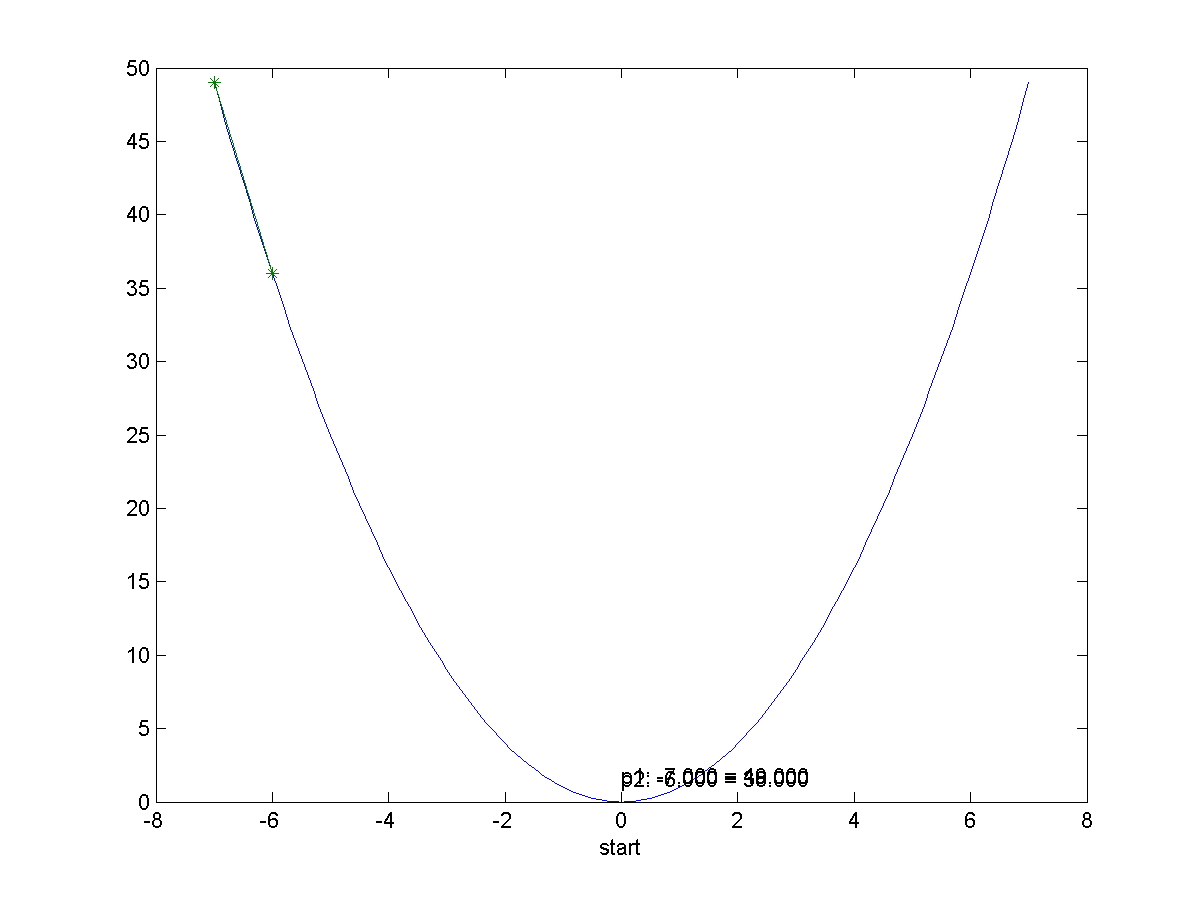
\includegraphics[height=0.75\paperheight]{../bilder/Quadrat/sinx_x001.png}
	\end{center}
\end{frame}

\begin{frame}{Minimum der Quadratfunktion}
\resizebox{1\textwidth}{!}{
\usetikzlibrary{shapes}
\begin{tikzpicture}[
  top/.style={draw,align=center,text width=5cm},
  med/.style={draw,align=center,text width=5cm},
  fin/.style={ellipse,draw,align=center}
]

\tikzstyle{level 1}=[sibling distance=150mm,align=center]
\tikzstyle{level 2}=[sibling distance=100mm,align=center]
\tikzstyle{level 3}=[sibling distance=80mm]


\node (start) at (0,1.5)[top] {$x_{max}$ am Mittelpunkt des restlichen Simplex ($x_m$) spiegeln $\rightarrow$ $x_{ref}$};

\node[top](top){$y_{ref}$ besser als  $y_{min}$?}
	child { node {Ja} child {child { child  { child { child {
		node[med] {Expansion: In Richtung $y_{ref}$ mit Faktor $\gamma$ Strecken  $\rightarrow y_{streck} $}
		child{
			node[med]  {$y_{streck}$ besser als $y_{min}$?}
			child { node {ja}
			child { node [fin]{$x_{max}$ mit $x_{streck}$ ersetzen} }}
			child { node {nein}
			child { node(a2) [fin]{$x_{max}$ mit $x_{ref}$ ersetzen} }}
		}
	}}}}}}
	child {
		node {Nein}
		child  {
		node [med] {$y_{ref}$ besser als zweitschlechtestes $y_i$ ?}
		child { node (b1) [] {Ja} }
		child { node {Nein} 
		child { node[med] {Ist $y_{ref}$ besser als $y_{max}$? }
			child {node{Nein}
				child { node (kont)[med] {Kontraktion: Rücke mit Faktor $\beta$ näher an Mittelpunkt $\rightarrow y_{kon}$ }
					child { node[med]  {Ist $y_{kon}$ besser als $y_{max}$?}
						child {node {Ja}
							child {node[fin] {Ersetze $x_{max}$ durch $x_{kon}$}}
						}
						child {node {Nein}
							child {node[fin] {Komprimierung: Rücke alle $x_i$ zu $x_{min}$ } }
						}
					}
				}
			}
			child {node {Ja}
				child { node (zukont)[med] {Ersetze $x_{max}$ durch $x_{ref}$ } }
			}
		}
		}
	}
	}
;
\draw (zukont) -- (kont);
\draw (b1) -- (a2);
\draw (start) --(top);

\end{tikzpicture}
}

\end{frame}


\begin{frame}{Minimum der Quadratfunktion}
	\begin{center}
		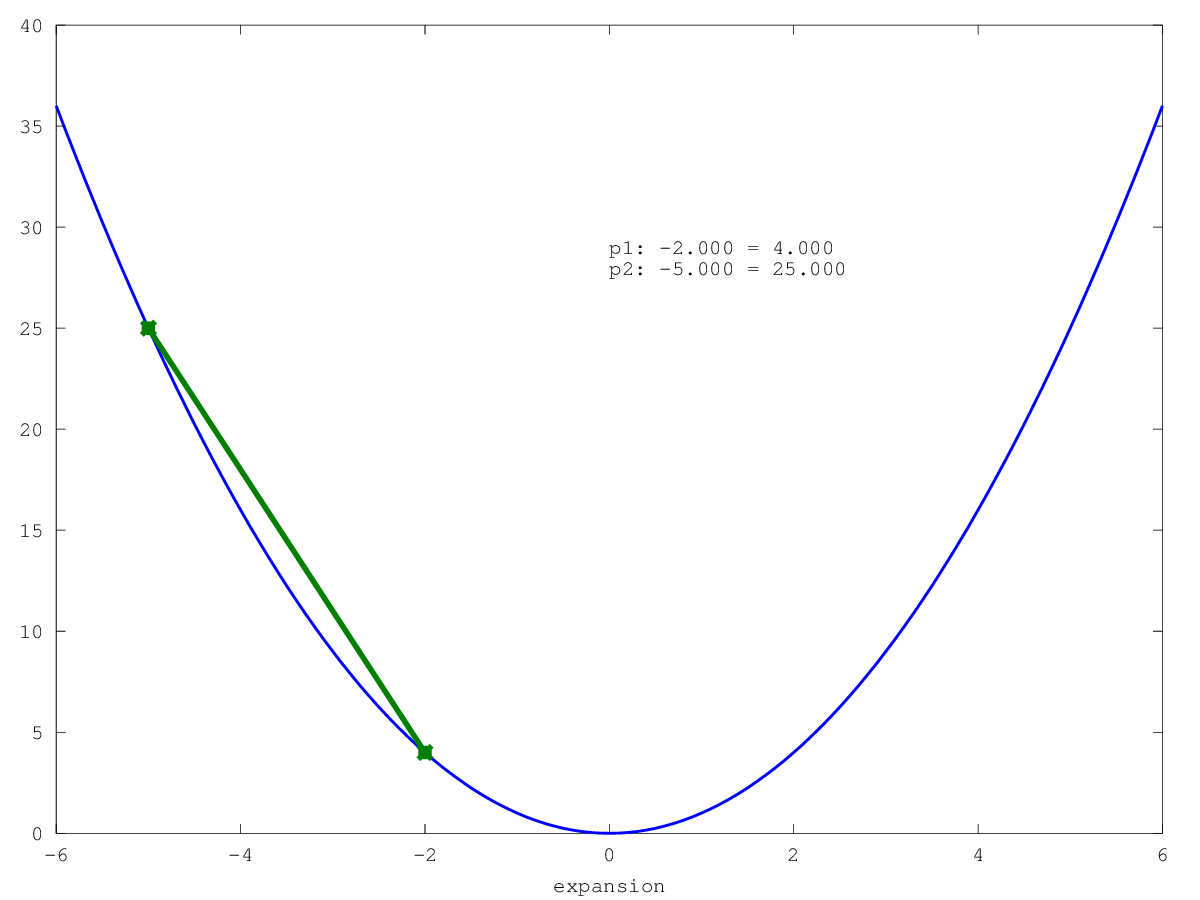
\includegraphics[height=0.75\paperheight]{../bilder/Quadrat/sinx_x002.png}
	\end{center}
\end{frame}
\begin{frame}{Minimum der Quadratfunktion}
	\begin{center}
		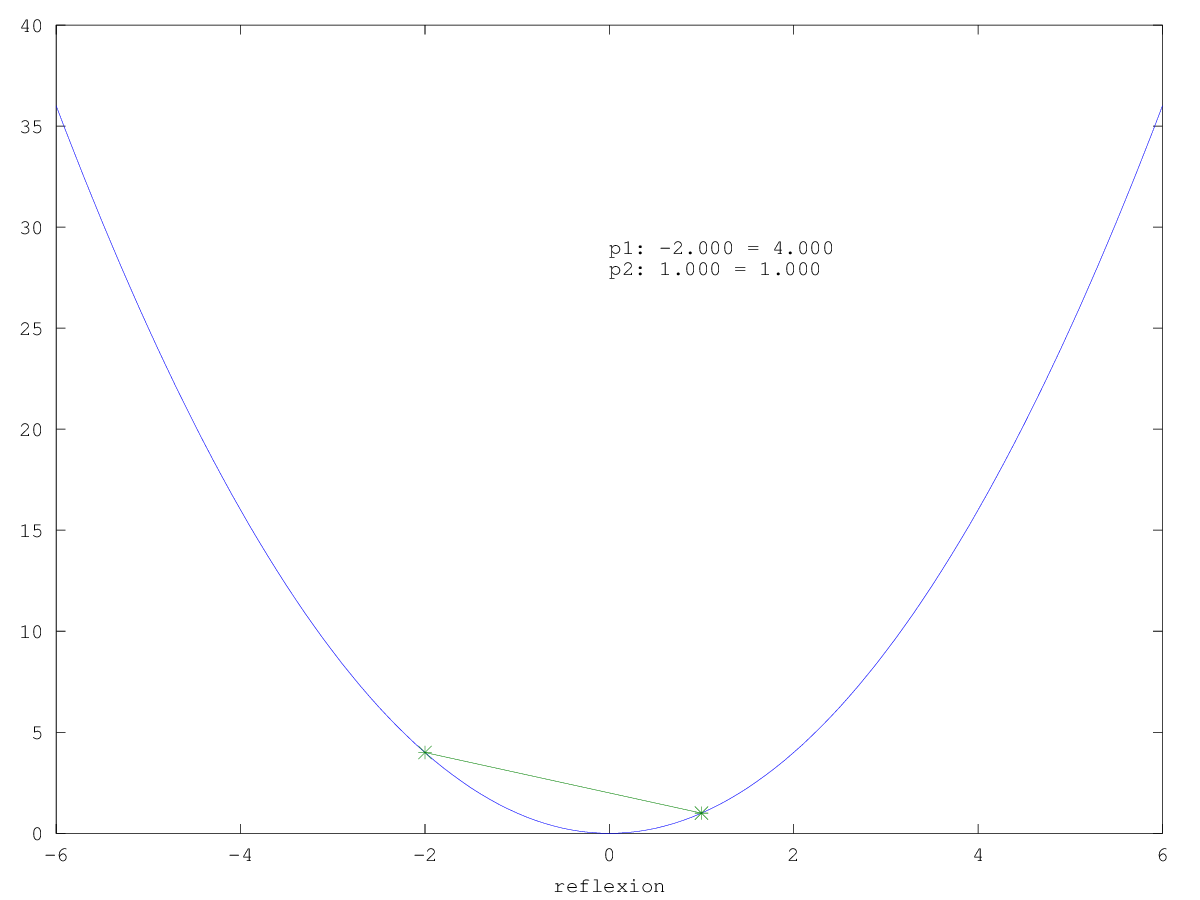
\includegraphics[height=0.75\paperheight]{../bilder/Quadrat/sinx_x003.png}
	\end{center}
\end{frame}
\begin{frame}{Minimum der Quadratfunktion}
	\begin{center}
		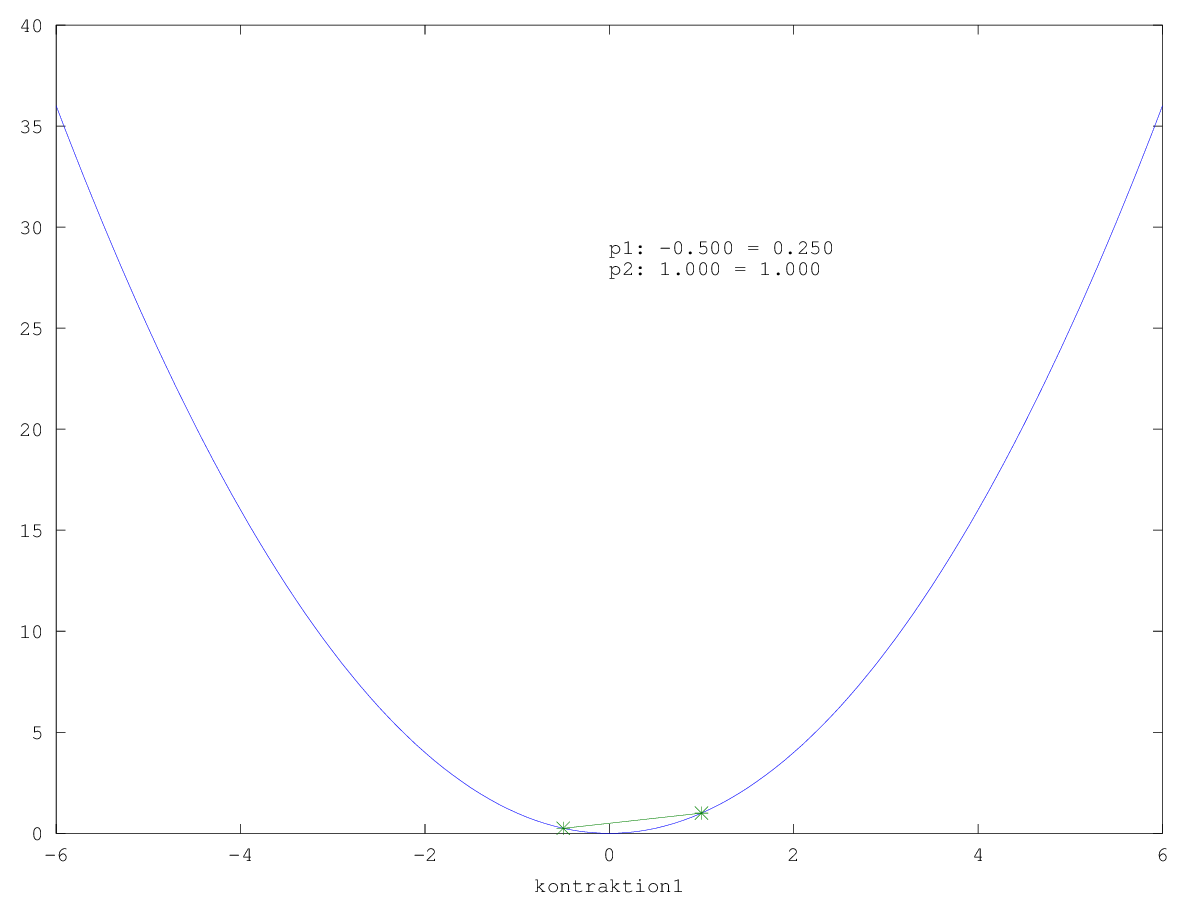
\includegraphics[height=0.75\paperheight]{../bilder/Quadrat/sinx_x004.png}
	\end{center}
\end{frame}
\begin{frame}{Minimum der Quadratfunktion}
	\begin{center}
		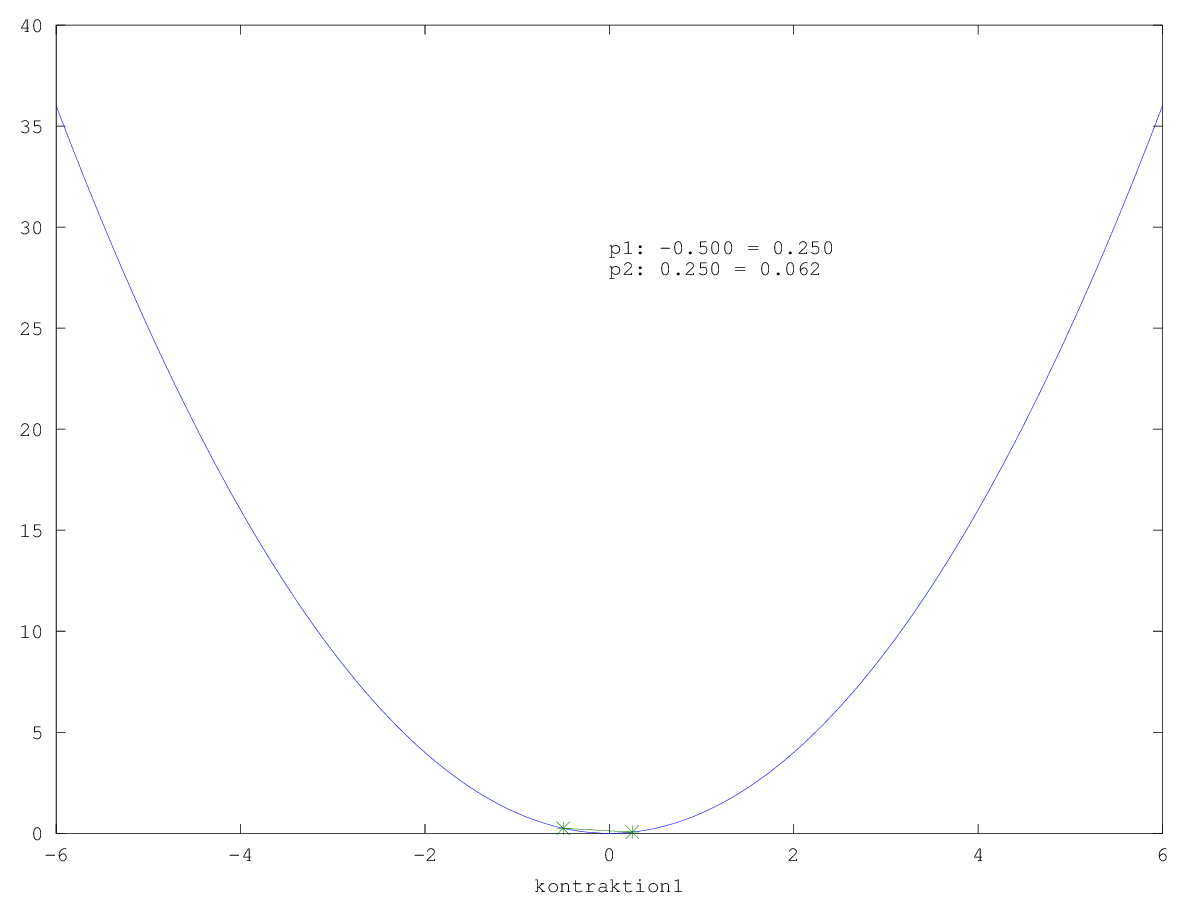
\includegraphics[height=0.75\paperheight]{../bilder/Quadrat/sinx_x005.png}
	\end{center}
\end{frame}
\begin{frame}{Minimum der Quadratfunktion}
	\begin{center}
		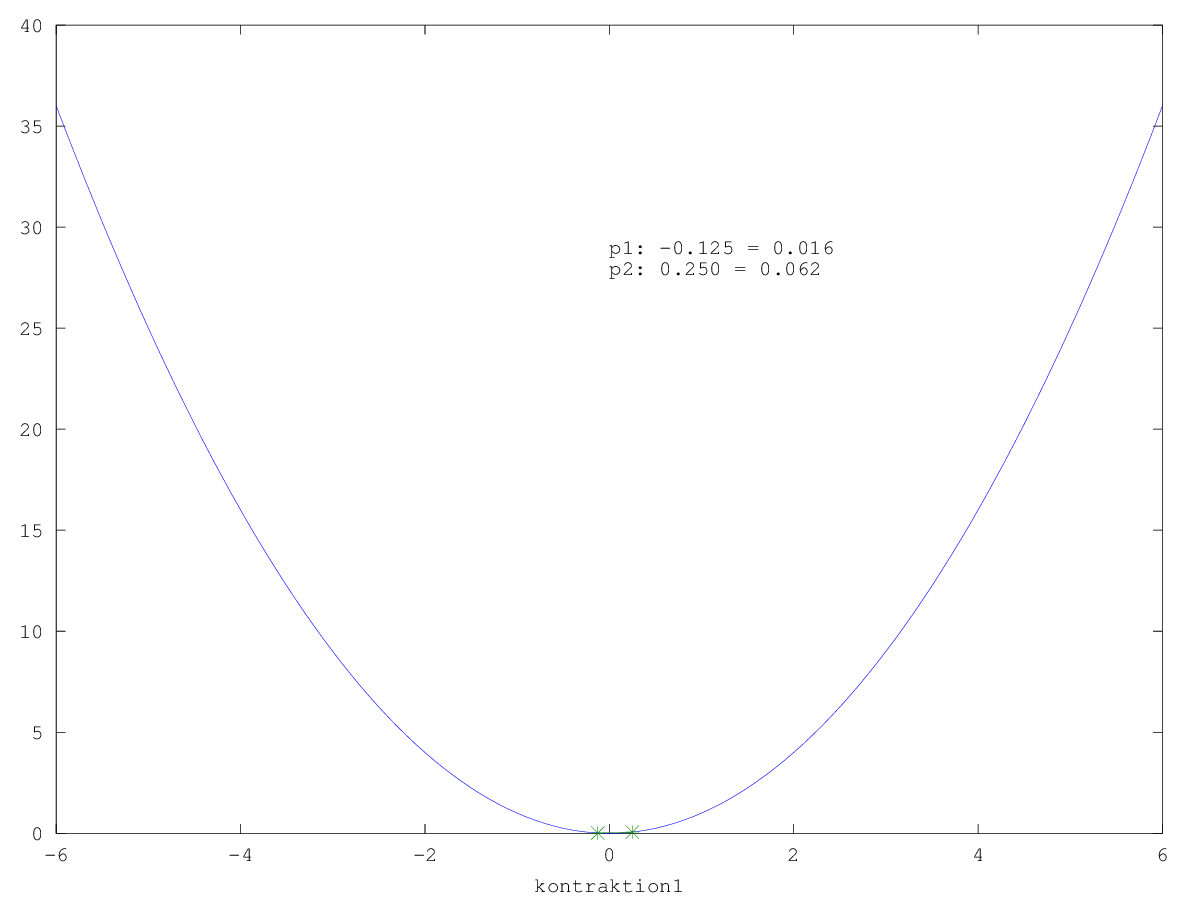
\includegraphics[height=0.75\paperheight]{../bilder/Quadrat/sinx_x006.png}
	\end{center}
\end{frame}
\begin{frame}{Minimum der Quadratfunktion}
	\begin{center}
		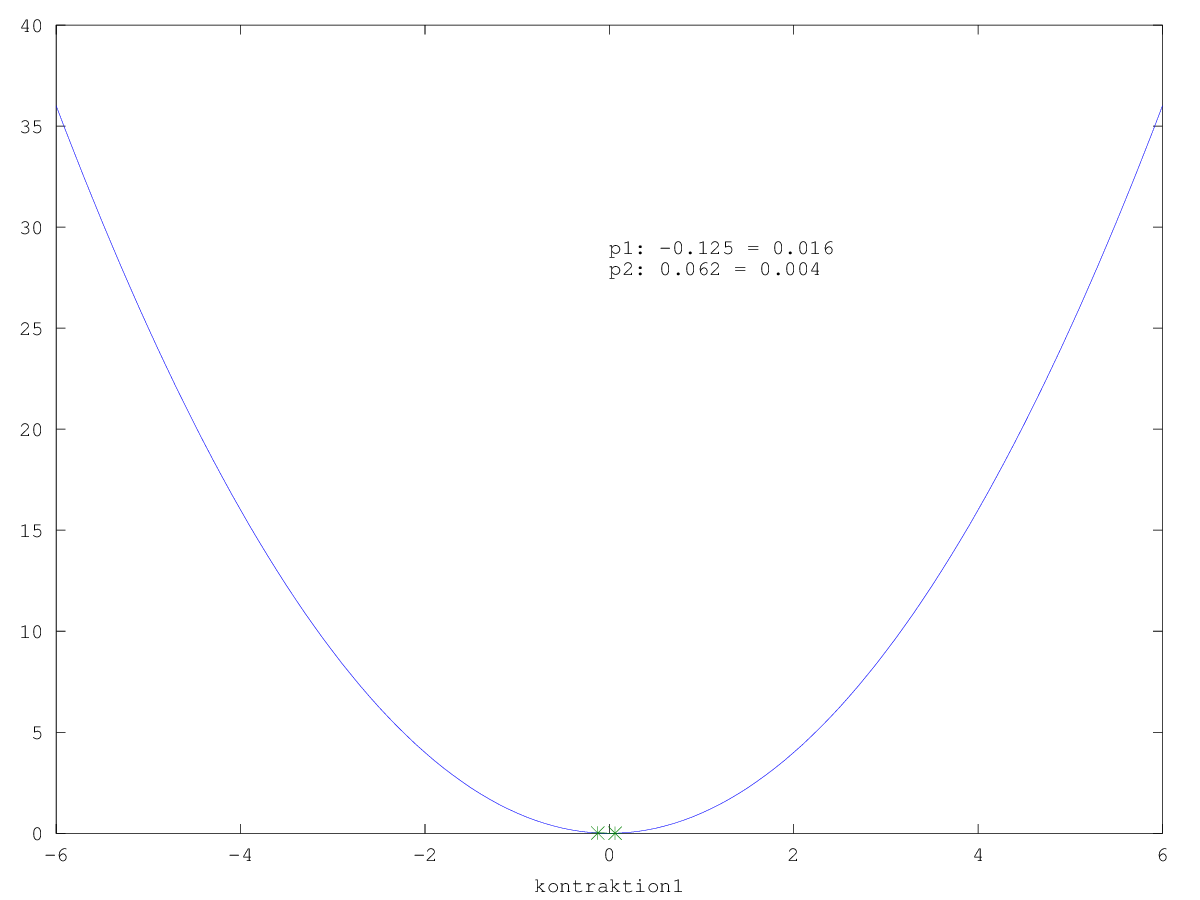
\includegraphics[height=0.75\paperheight]{../bilder/Quadrat/sinx_x007.png}
	\end{center}
\end{frame}
\begin{frame}{Minimum der Quadratfunktion}
	\begin{center}
		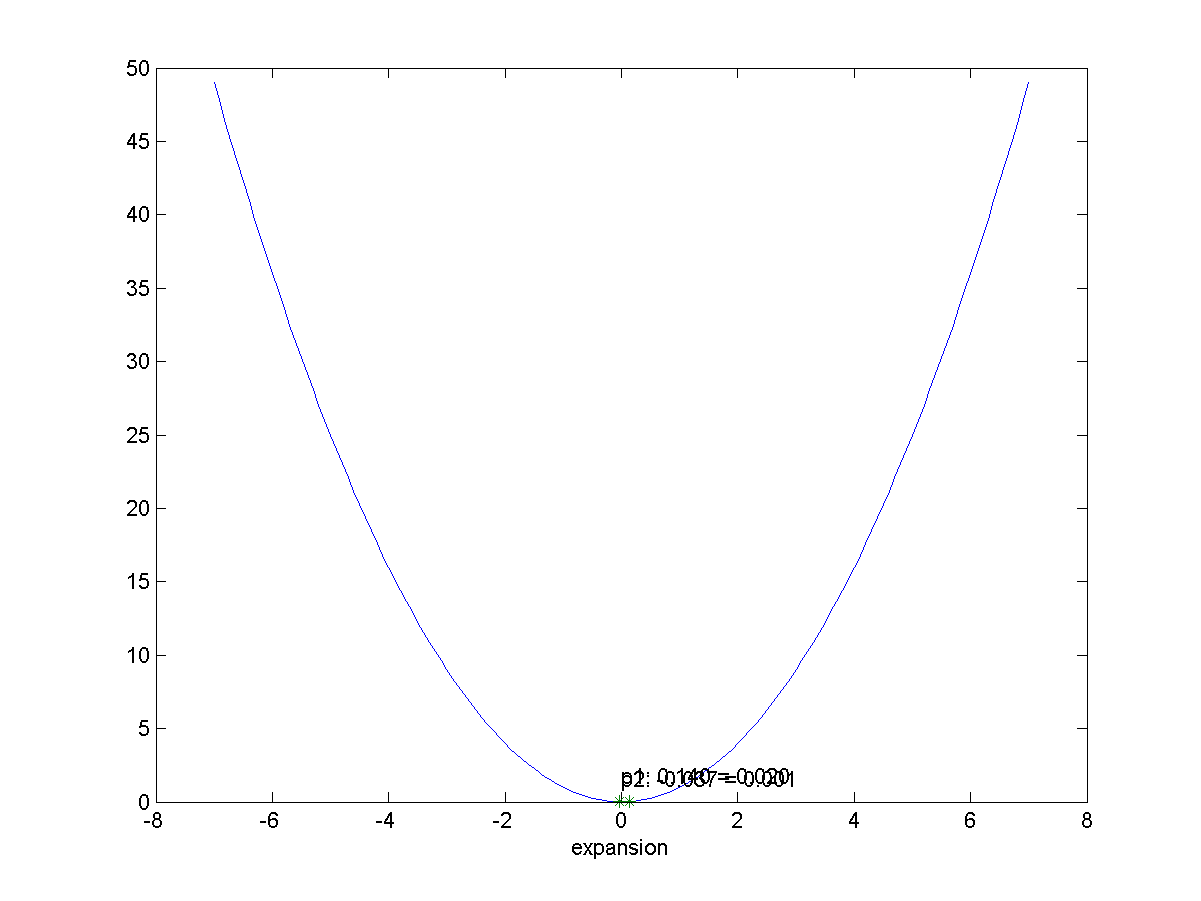
\includegraphics[height=0.75\paperheight]{../bilder/Quadrat/sinx_x008.png}
	\end{center}
\end{frame}
\begin{frame}{Minimum der Quadratfunktion}
	\begin{center}
		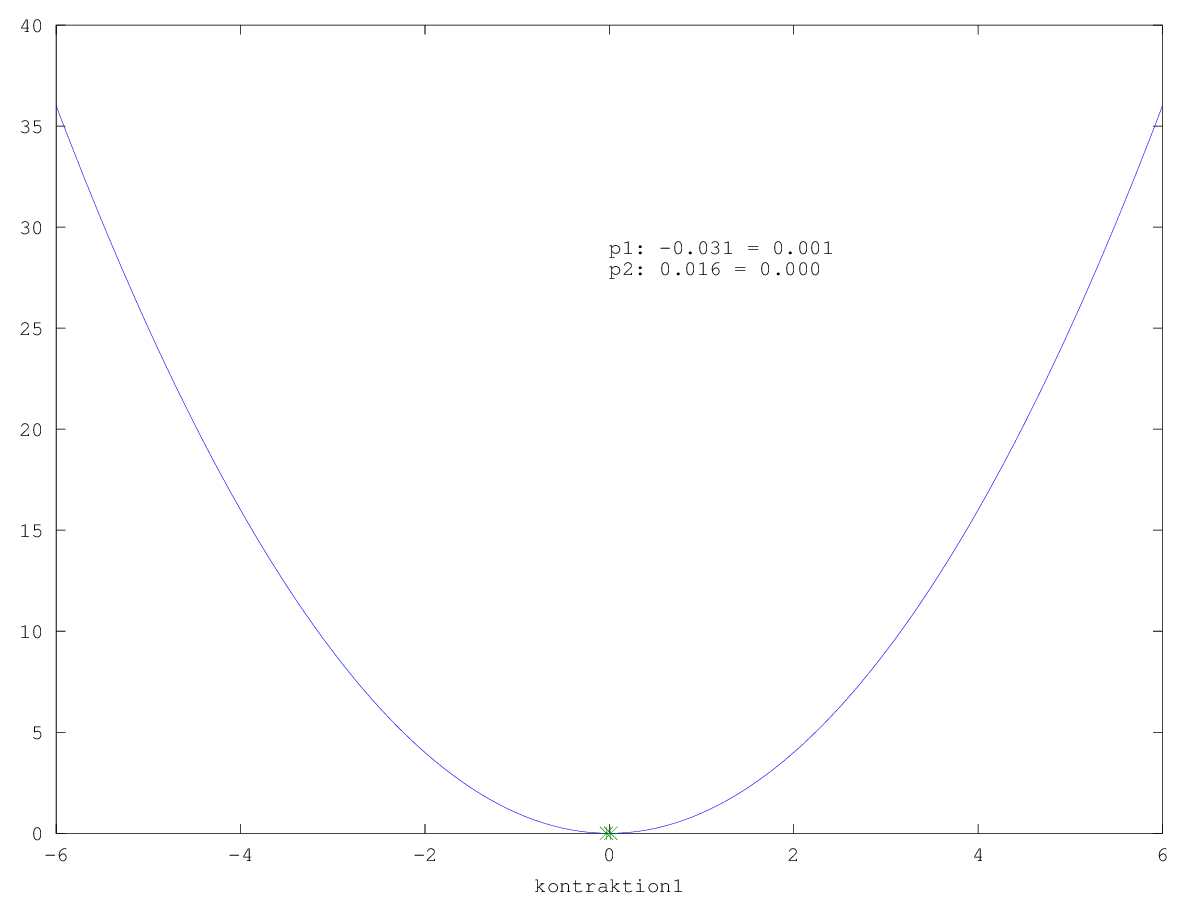
\includegraphics[height=0.75\paperheight]{../bilder/Quadrat/sinx_x009.png}
	\end{center}
\end{frame}
\begin{frame}{Minimum der Quadratfunktion}
	\begin{center}
		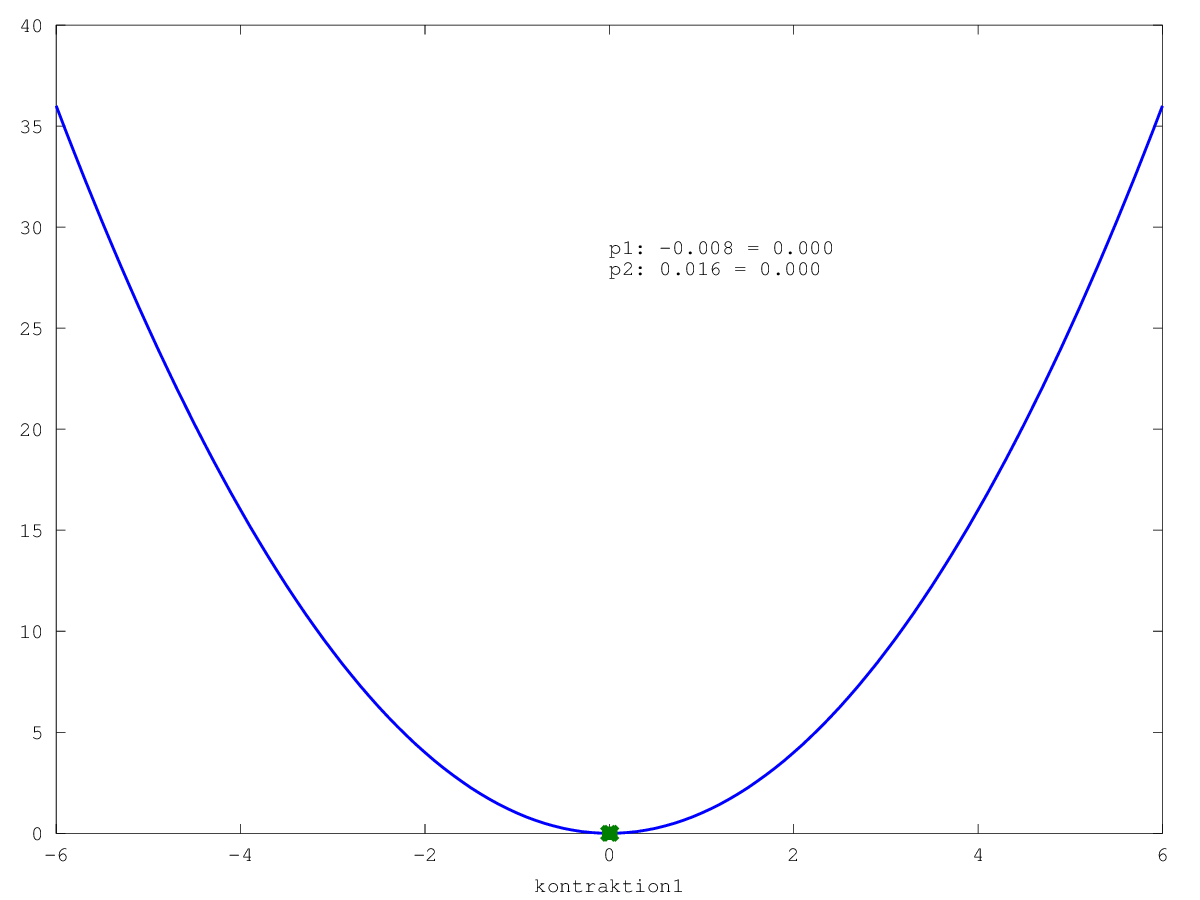
\includegraphics[height=0.75\paperheight]{../bilder/Quadrat/sinx_x010.png}
	\end{center}
\end{frame}









\begin{frame}{Weiteres Beispiel}
	\begin{center}
		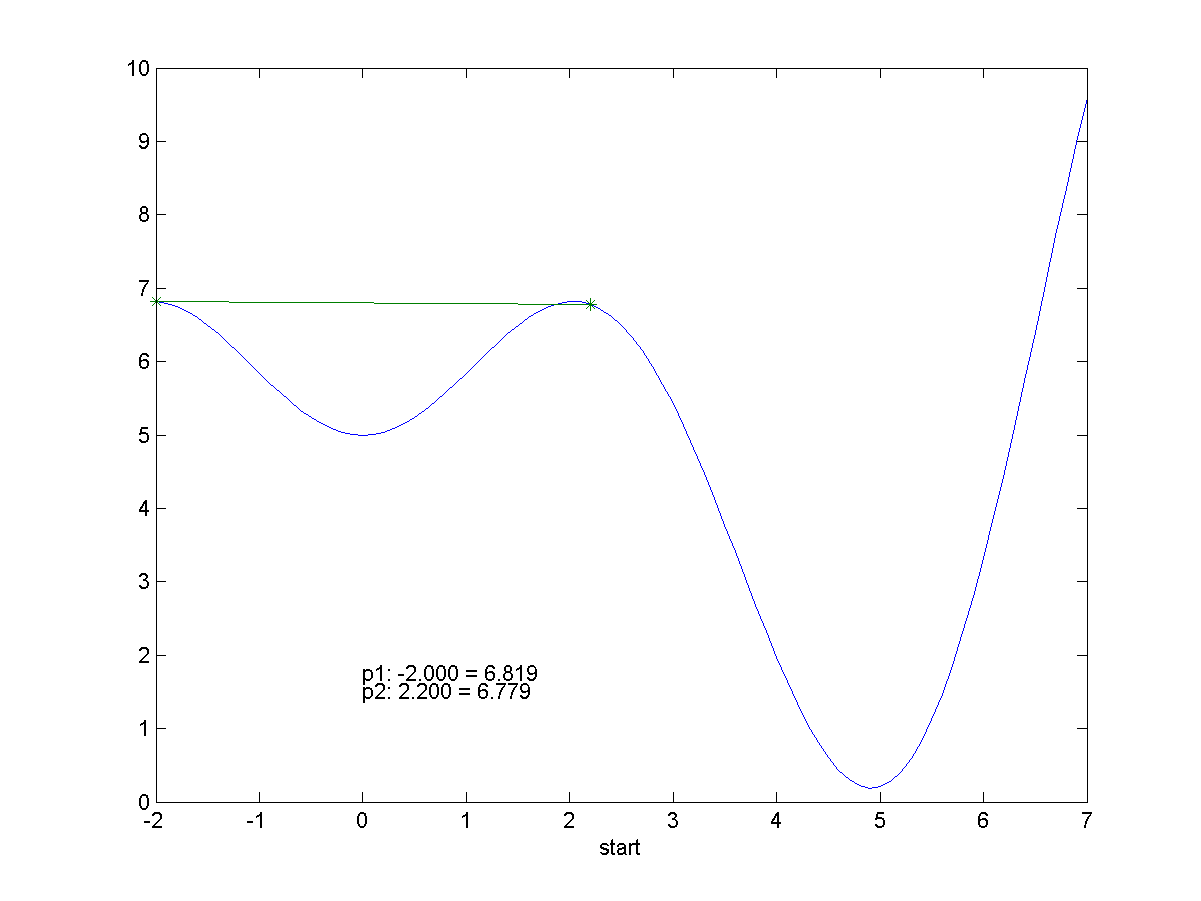
\includegraphics[height=0.75\paperheight]{../bilder/GlobMinima/sinx_x001.png}
	\end{center}
\end{frame}
\begin{frame}{Weiteres Beispiel}
	\begin{center}
		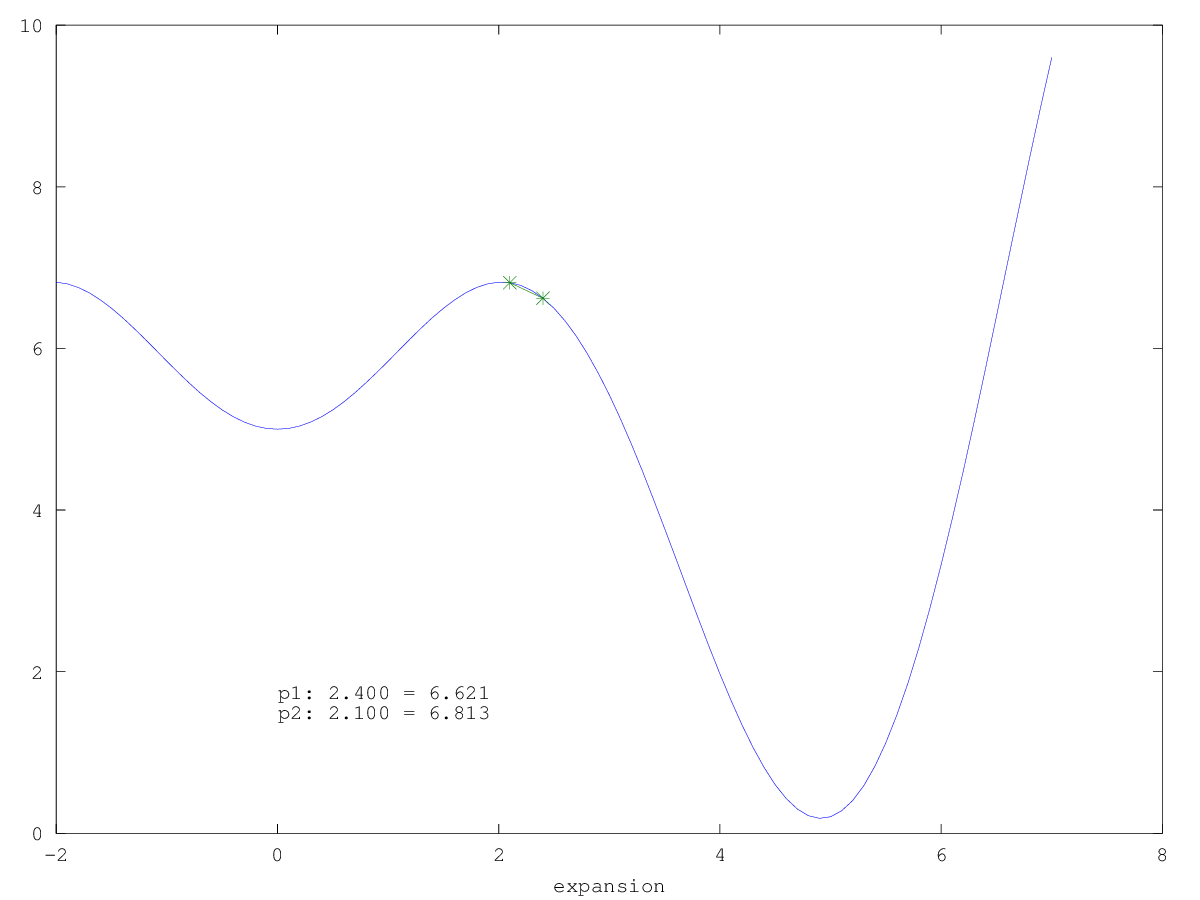
\includegraphics[height=0.75\paperheight]{../bilder/GlobMinima/sinx_x002.png}
	\end{center}
\end{frame}
\begin{frame}{Weiteres Beispiel}
	\begin{center}
		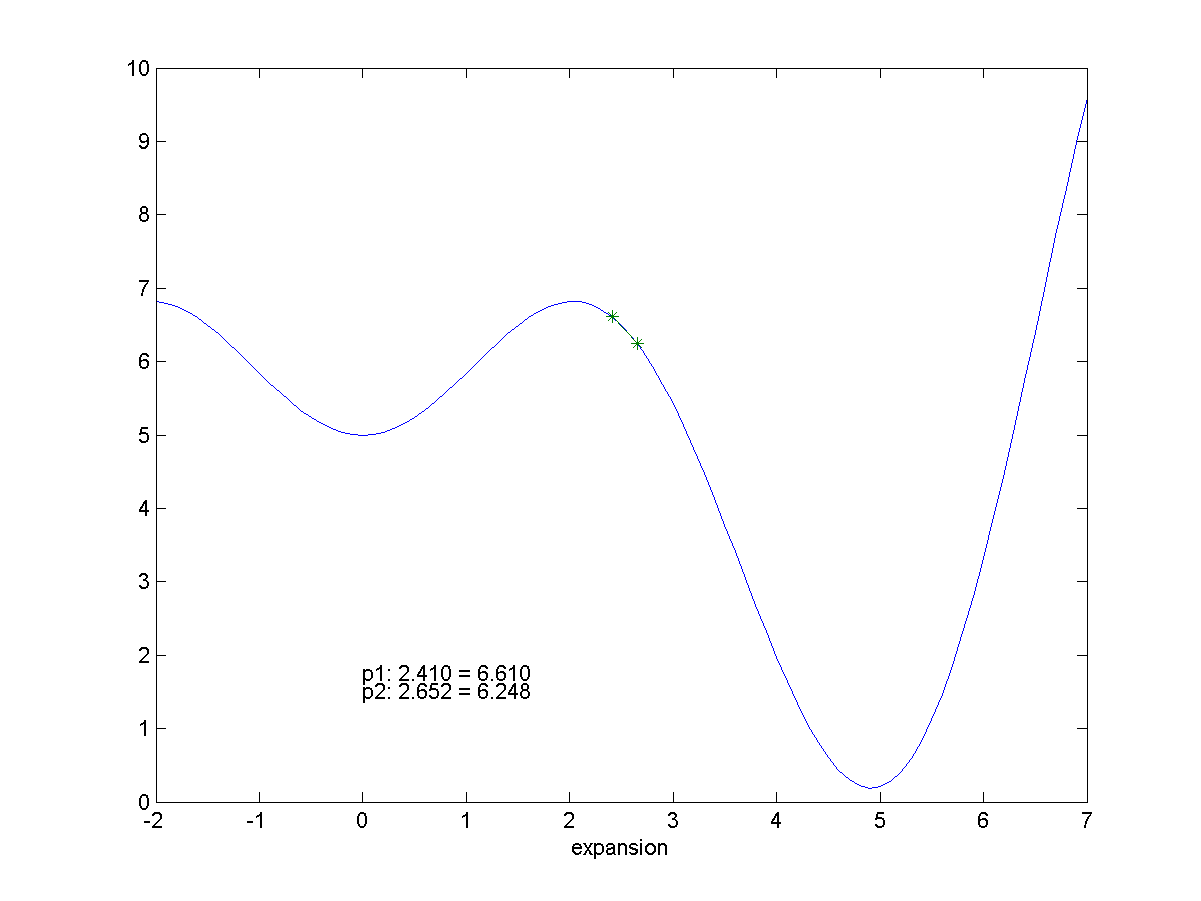
\includegraphics[height=0.75\paperheight]{../bilder/GlobMinima/sinx_x003.png}
	\end{center}
\end{frame}
\begin{frame}{Weiteres Beispiel}
	\begin{center}
		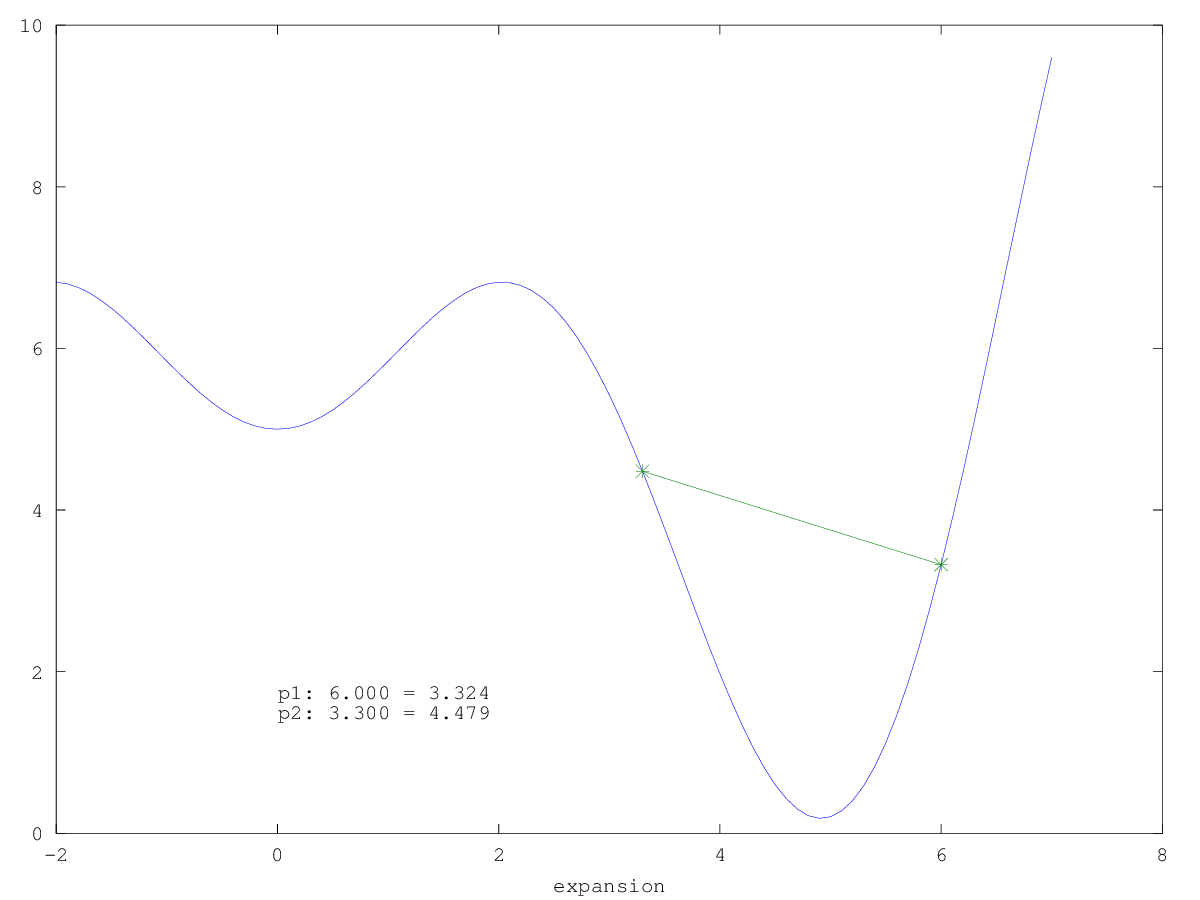
\includegraphics[height=0.75\paperheight]{../bilder/GlobMinima/sinx_x004.png}
	\end{center}
\end{frame}
\begin{frame}{Weiteres Beispiel}
	\begin{center}
		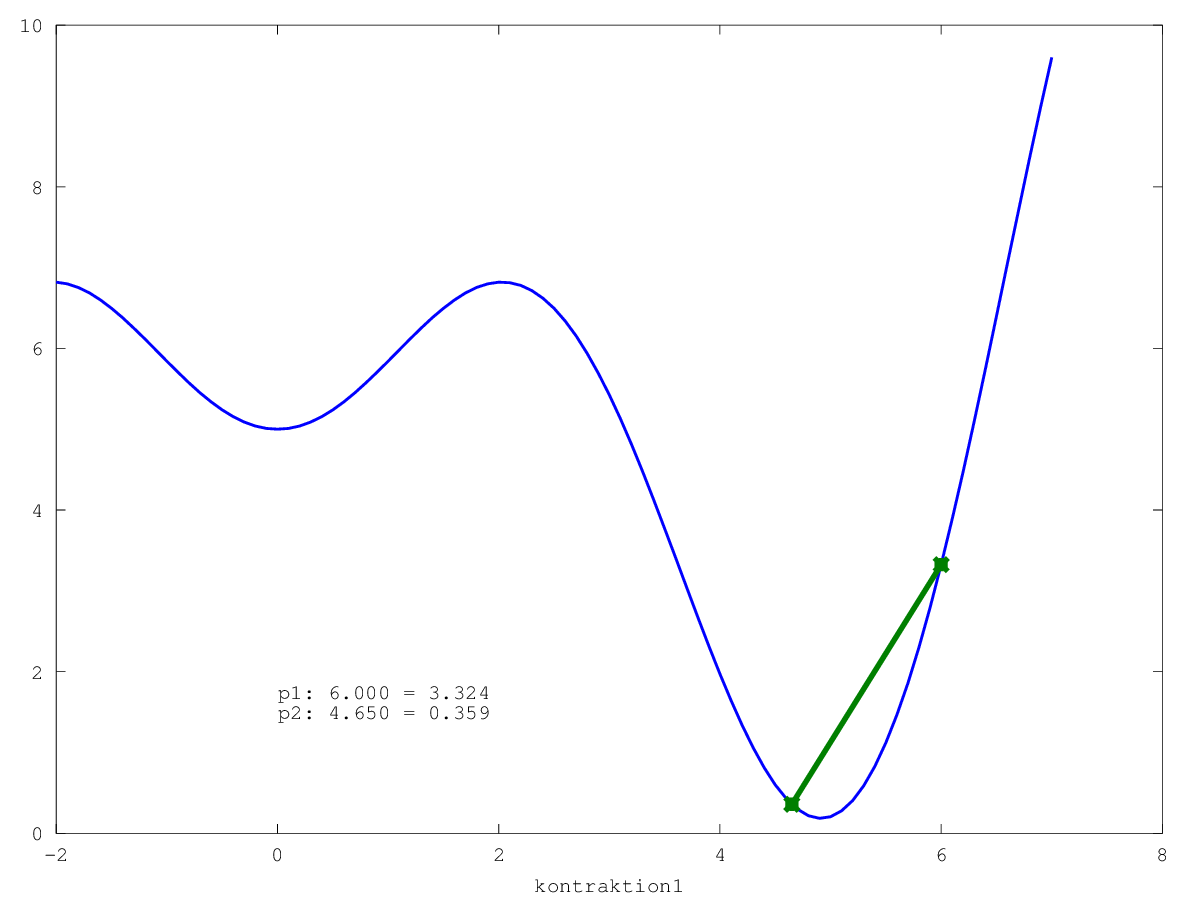
\includegraphics[height=0.75\paperheight]{../bilder/GlobMinima/sinx_x005.png}
	\end{center}
\end{frame}
\begin{frame}{Weiteres Beispiel}
	\begin{center}
		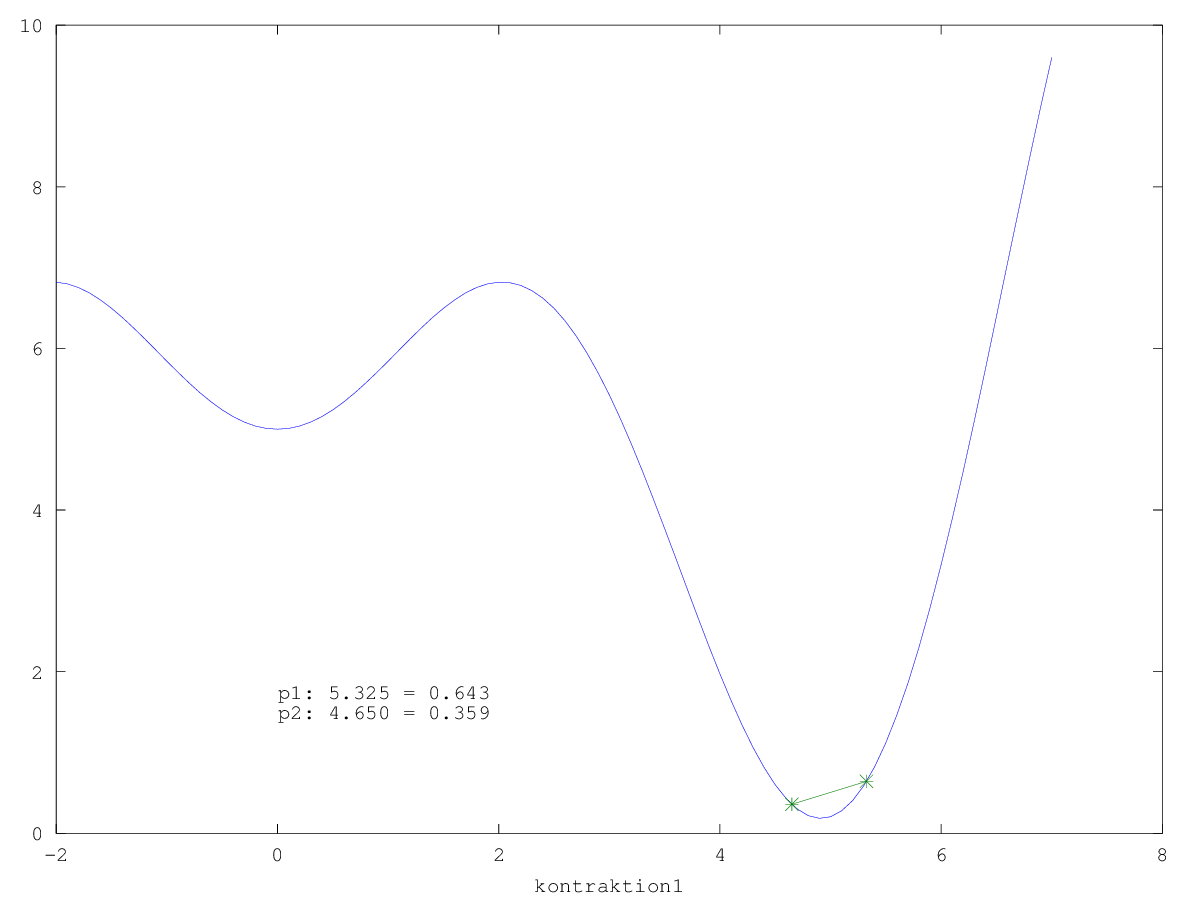
\includegraphics[height=0.75\paperheight]{../bilder/GlobMinima/sinx_x006.png}
	\end{center}
\end{frame}
\begin{frame}{Weiteres Beispiel}
	\begin{center}
		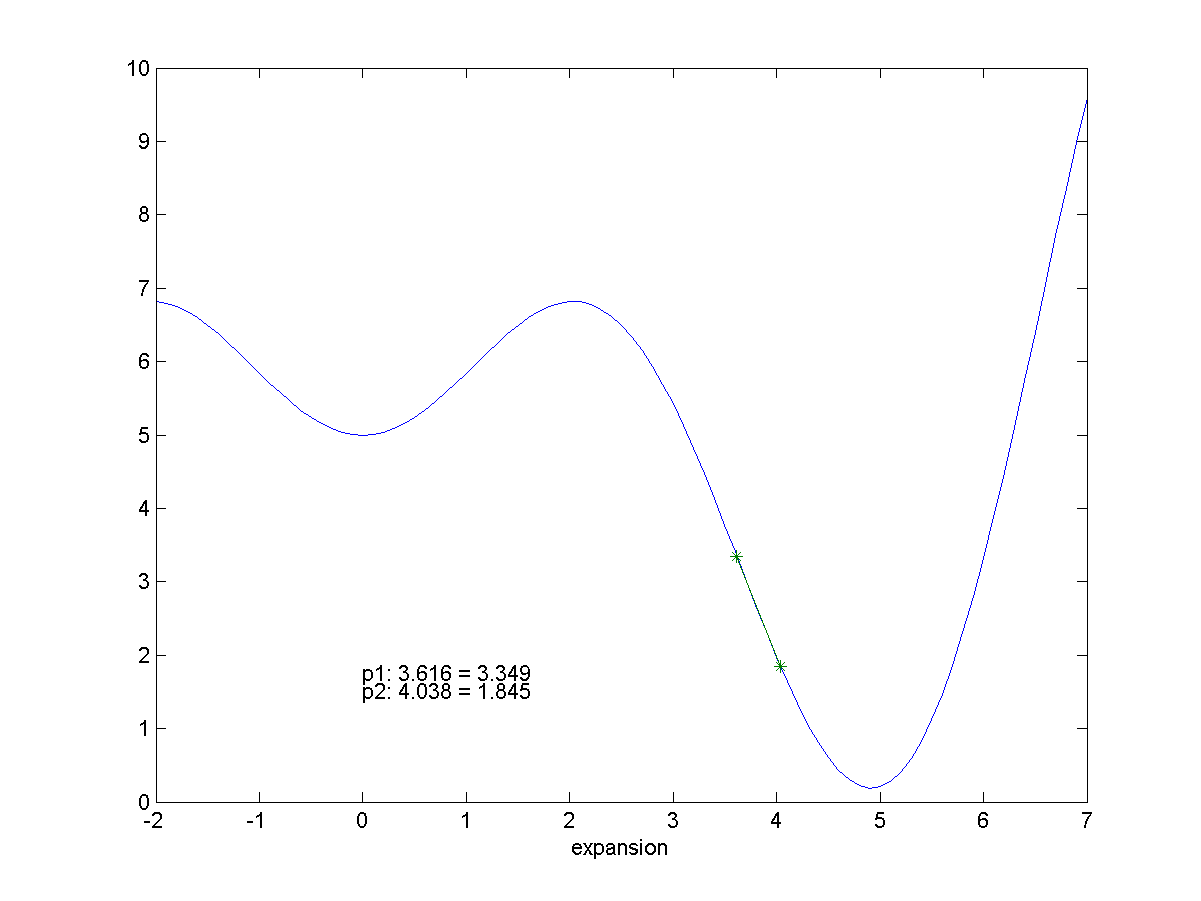
\includegraphics[height=0.75\paperheight]{../bilder/GlobMinima/sinx_x007.png}
	\end{center}
\end{frame}
\begin{frame}{Weiteres Beispiel}
	\begin{center}
		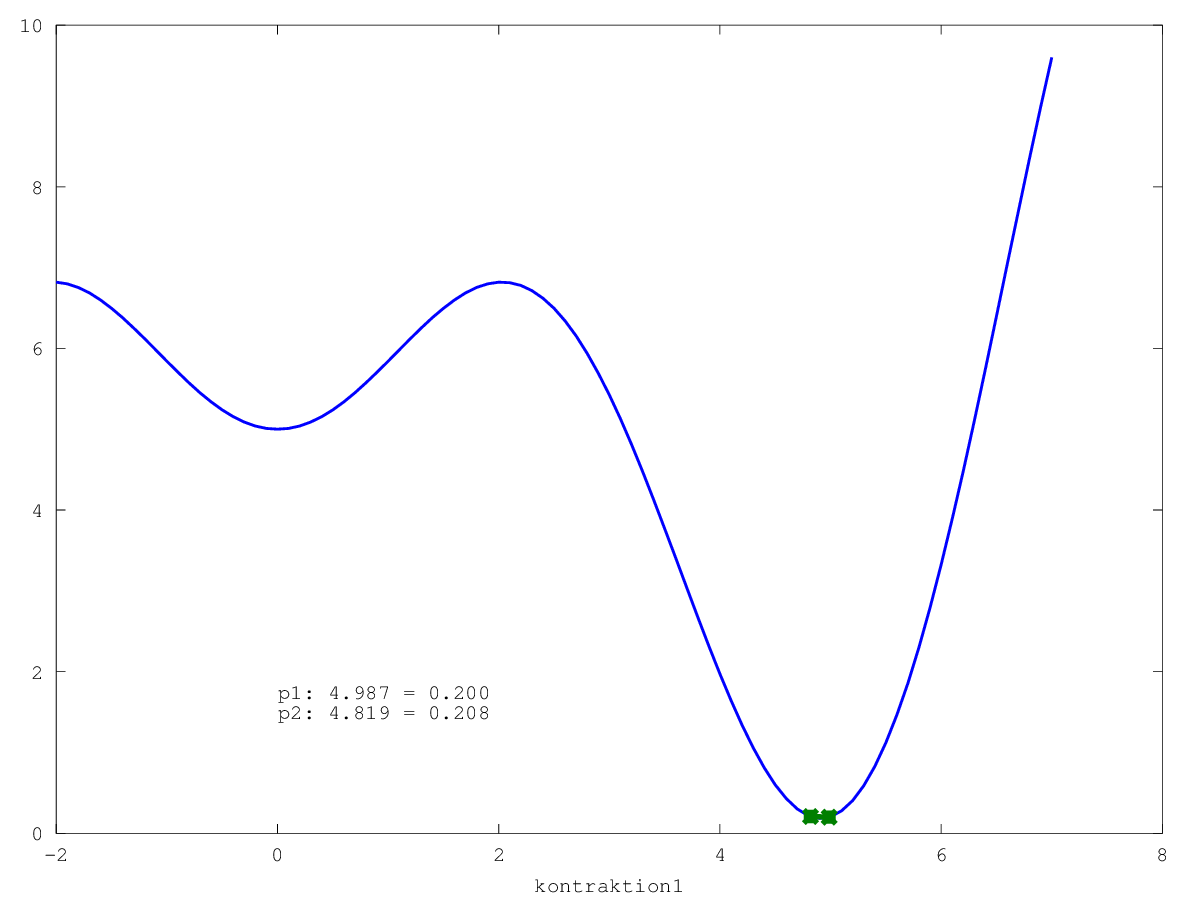
\includegraphics[height=0.75\paperheight]{../bilder/GlobMinima/sinx_x008.png}
	\end{center}
\end{frame}
\begin{frame}{Weiteres Beispiel}
	\begin{center}
		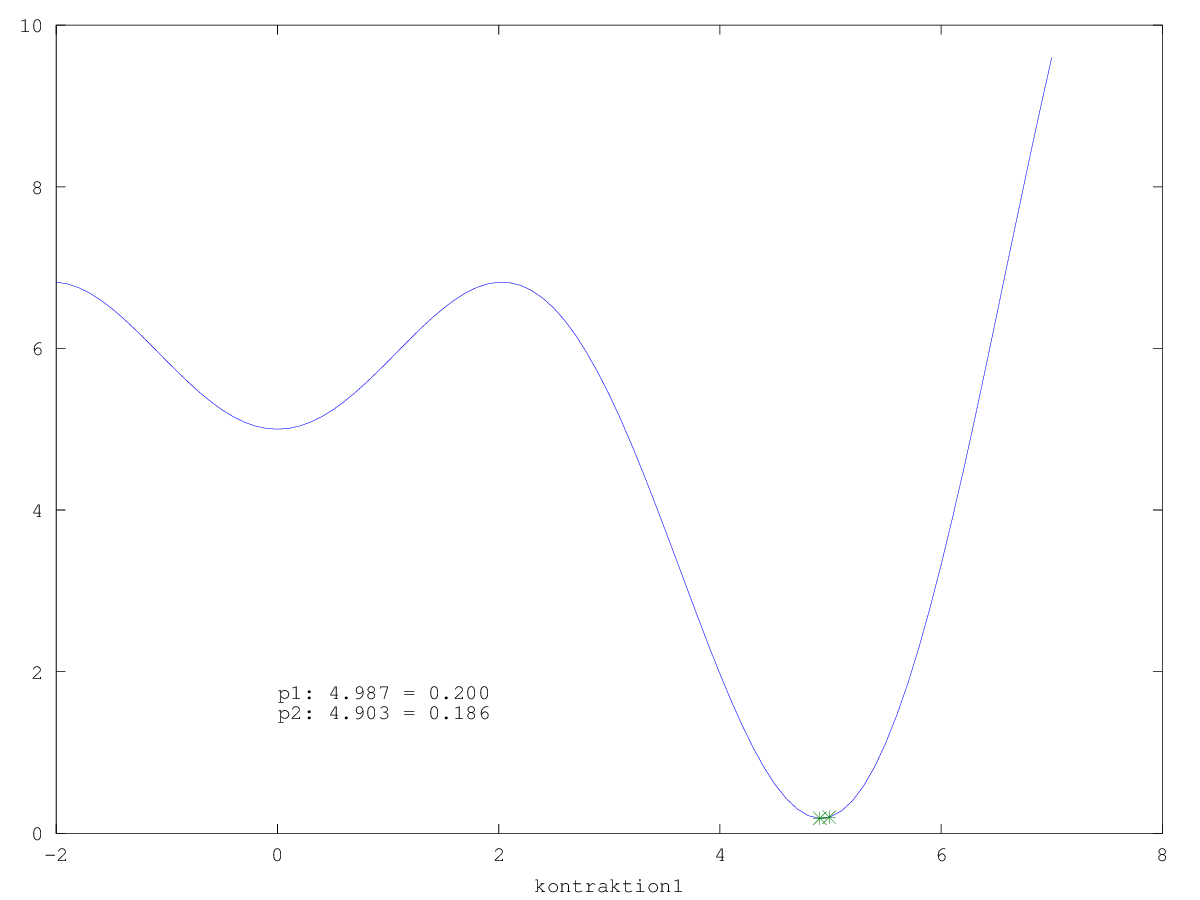
\includegraphics[height=0.75\paperheight]{../bilder/GlobMinima/sinx_x009.png}
	\end{center}
\end{frame}
\begin{frame}{Weiteres Beispiel}
	\begin{center}
		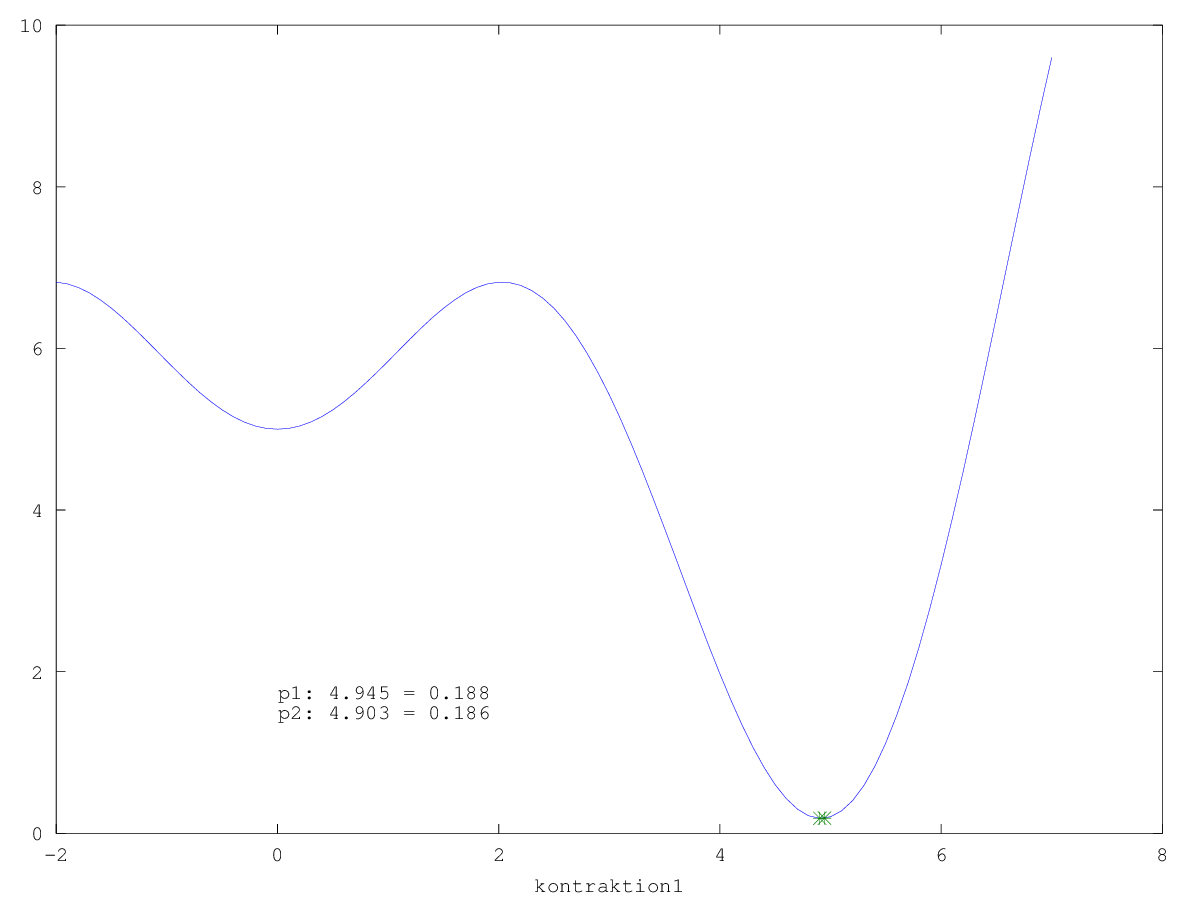
\includegraphics[height=0.75\paperheight]{../bilder/GlobMinima/sinx_x010.png}
	\end{center}
\end{frame}










\section{Probleme}
\begin{frame}{Programm}\tableofcontents[currentsection]\end{frame}
\begin{frame}{Probleme}
	\begin{center}
		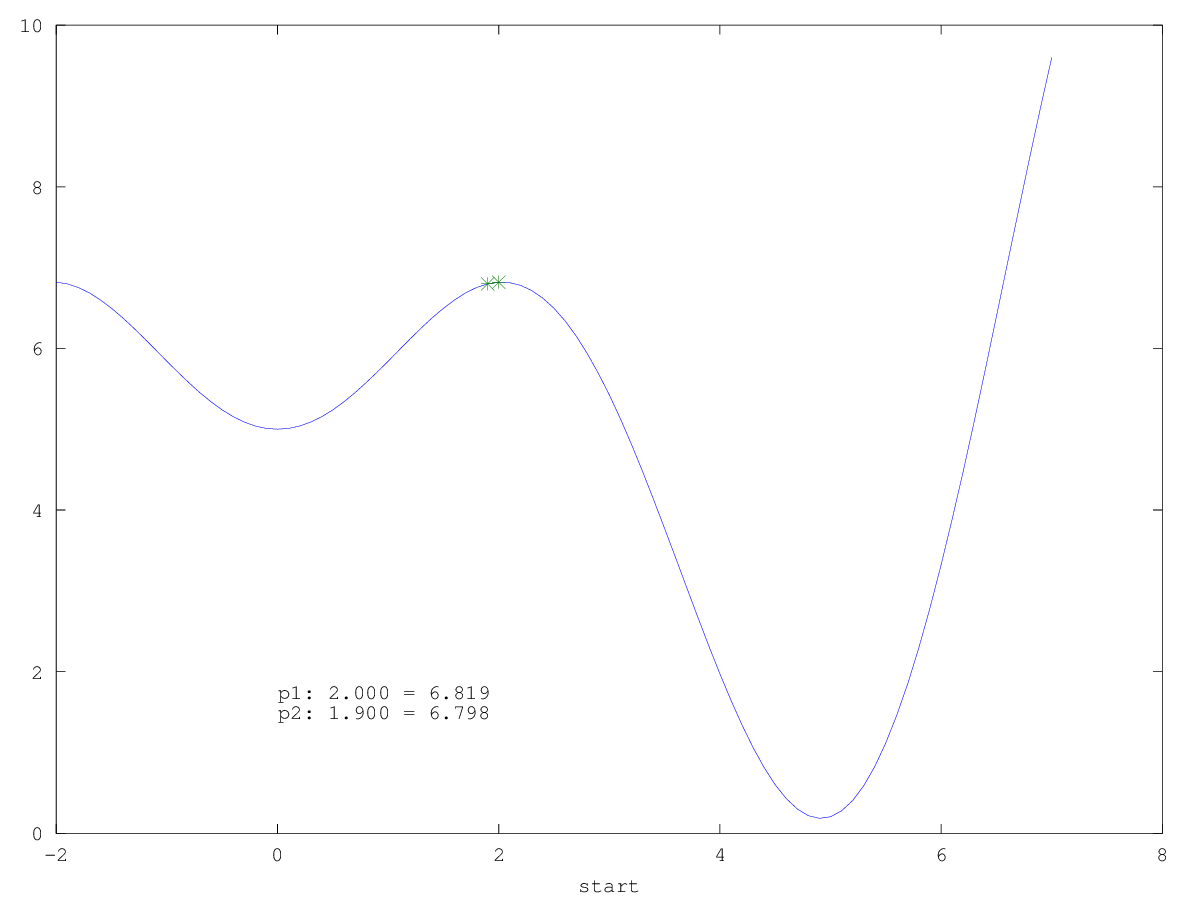
\includegraphics[height=0.75\paperheight]{../bilder/LokMinima/sinx_x001.png}
	\end{center}
\end{frame}
\begin{frame}{Probleme}
	\begin{center}
		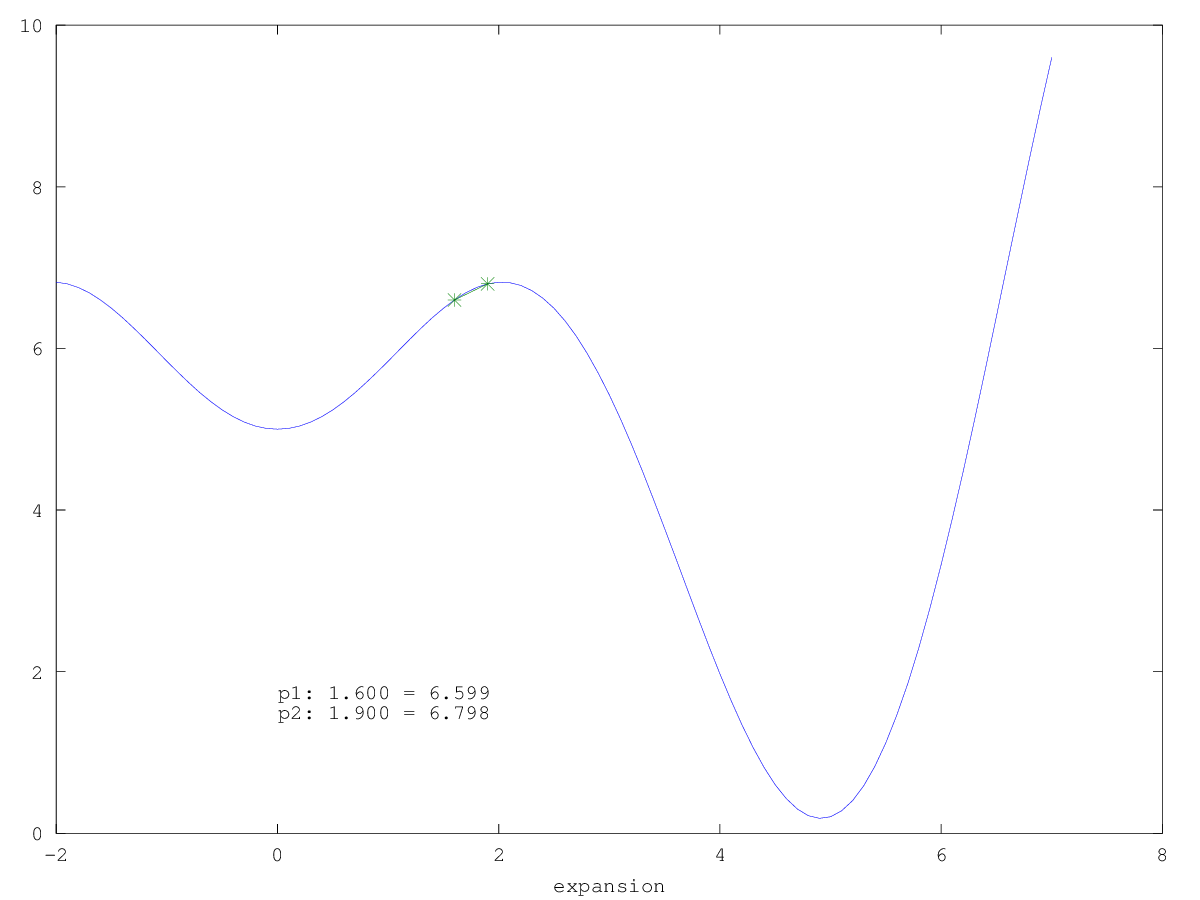
\includegraphics[height=0.75\paperheight]{../bilder/LokMinima/sinx_x002.png}
	\end{center}
\end{frame}
\begin{frame}{Probleme}
	\begin{center}
		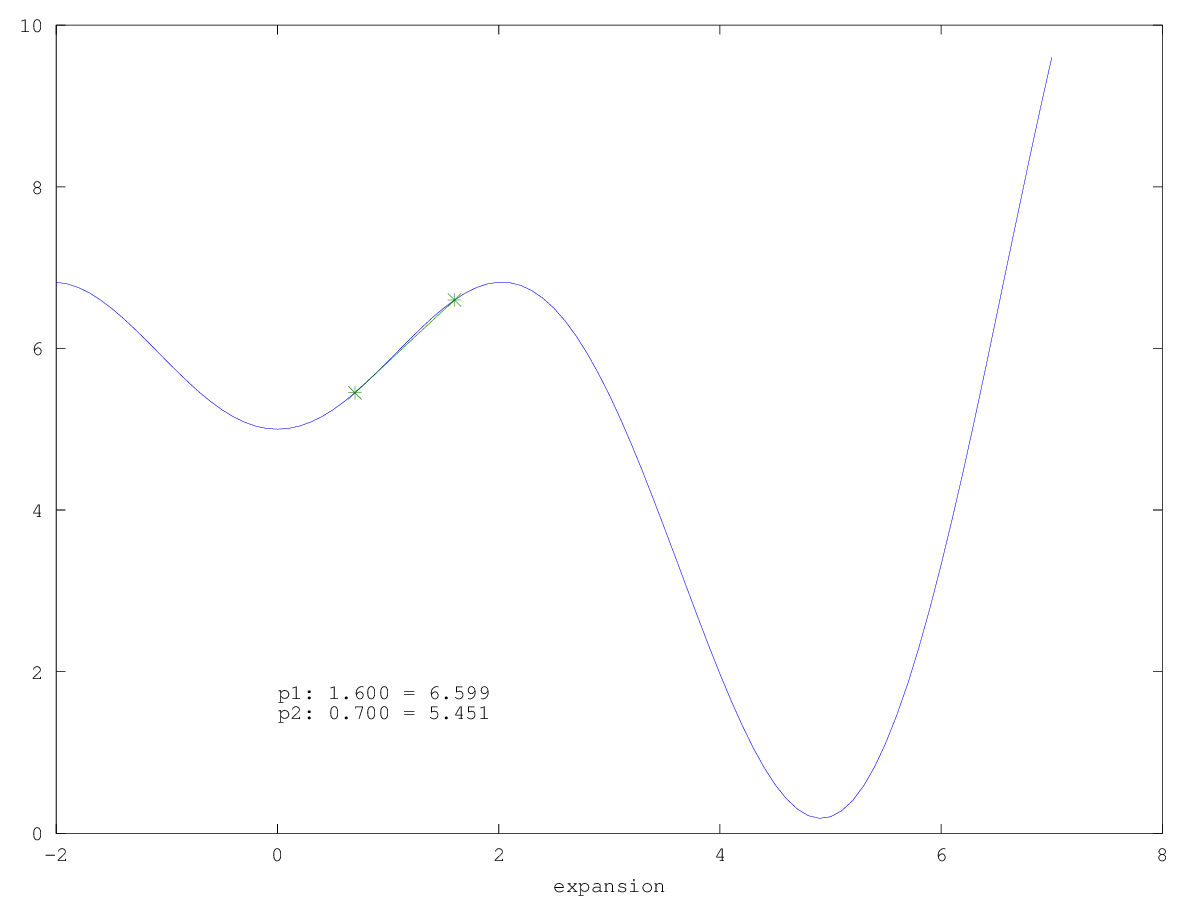
\includegraphics[height=0.75\paperheight]{../bilder/LokMinima/sinx_x003.png}
	\end{center}
\end{frame}
\begin{frame}{Probleme}
	\begin{center}
		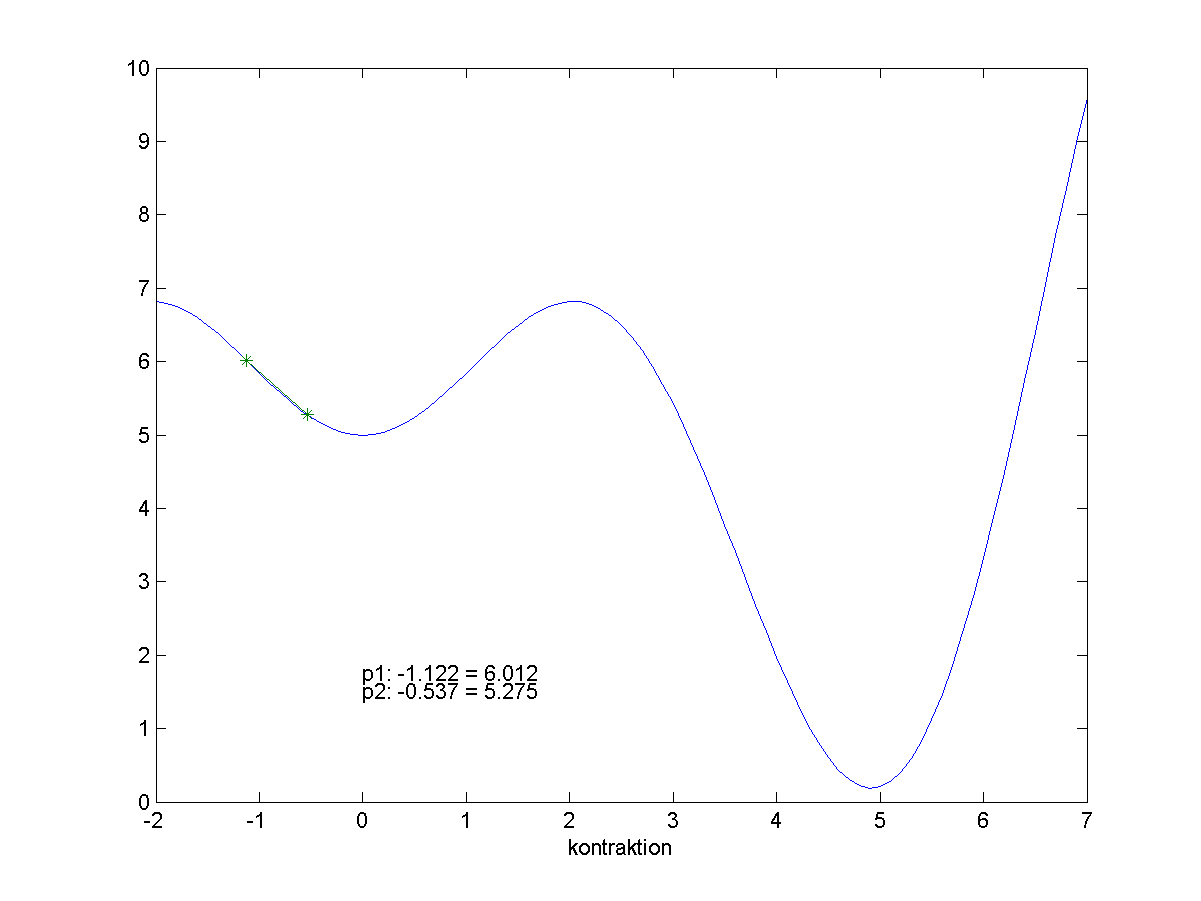
\includegraphics[height=0.75\paperheight]{../bilder/LokMinima/sinx_x004.png}
	\end{center}
\end{frame}
\begin{frame}{Probleme}
	\begin{center}
		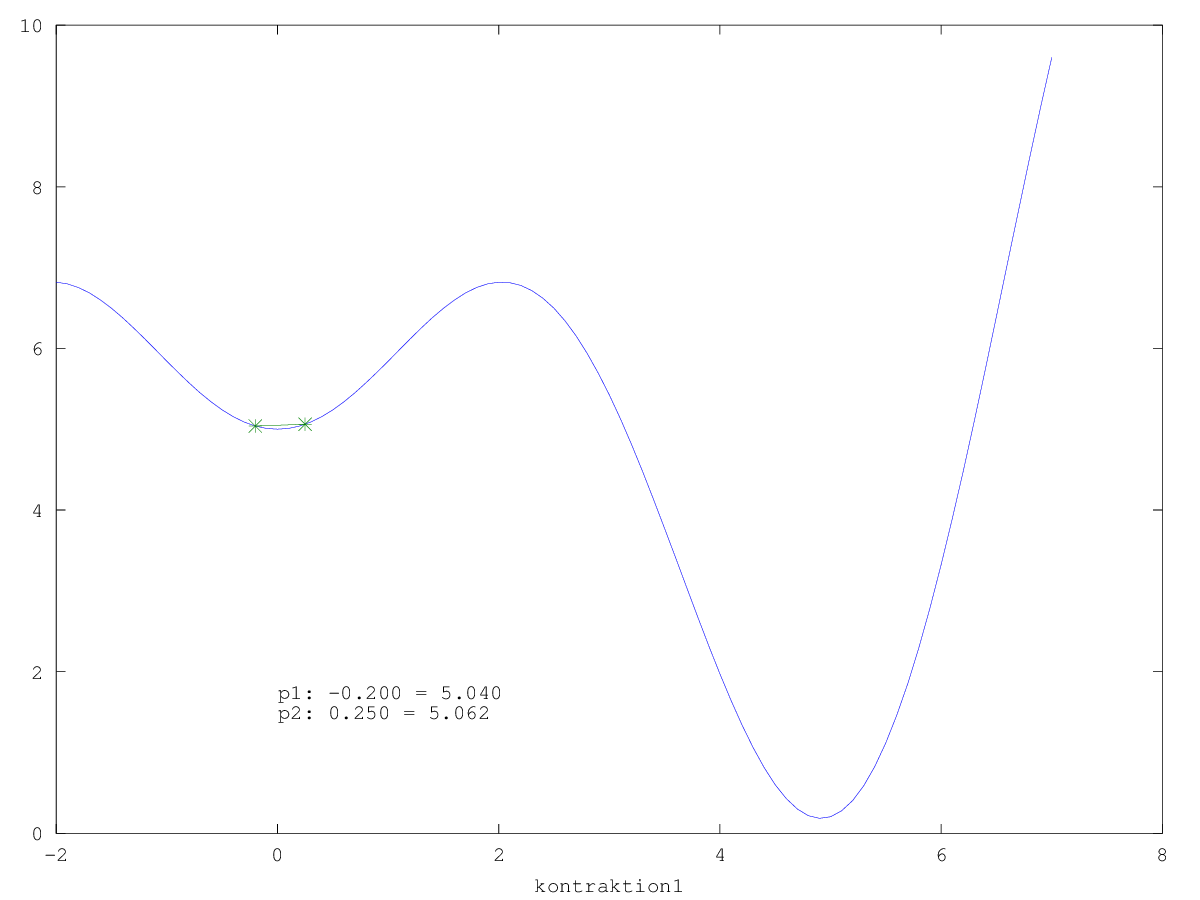
\includegraphics[height=0.75\paperheight]{../bilder/LokMinima/sinx_x005.png}
	\end{center}
\end{frame}
\begin{frame}{Probleme}
	\begin{center}
		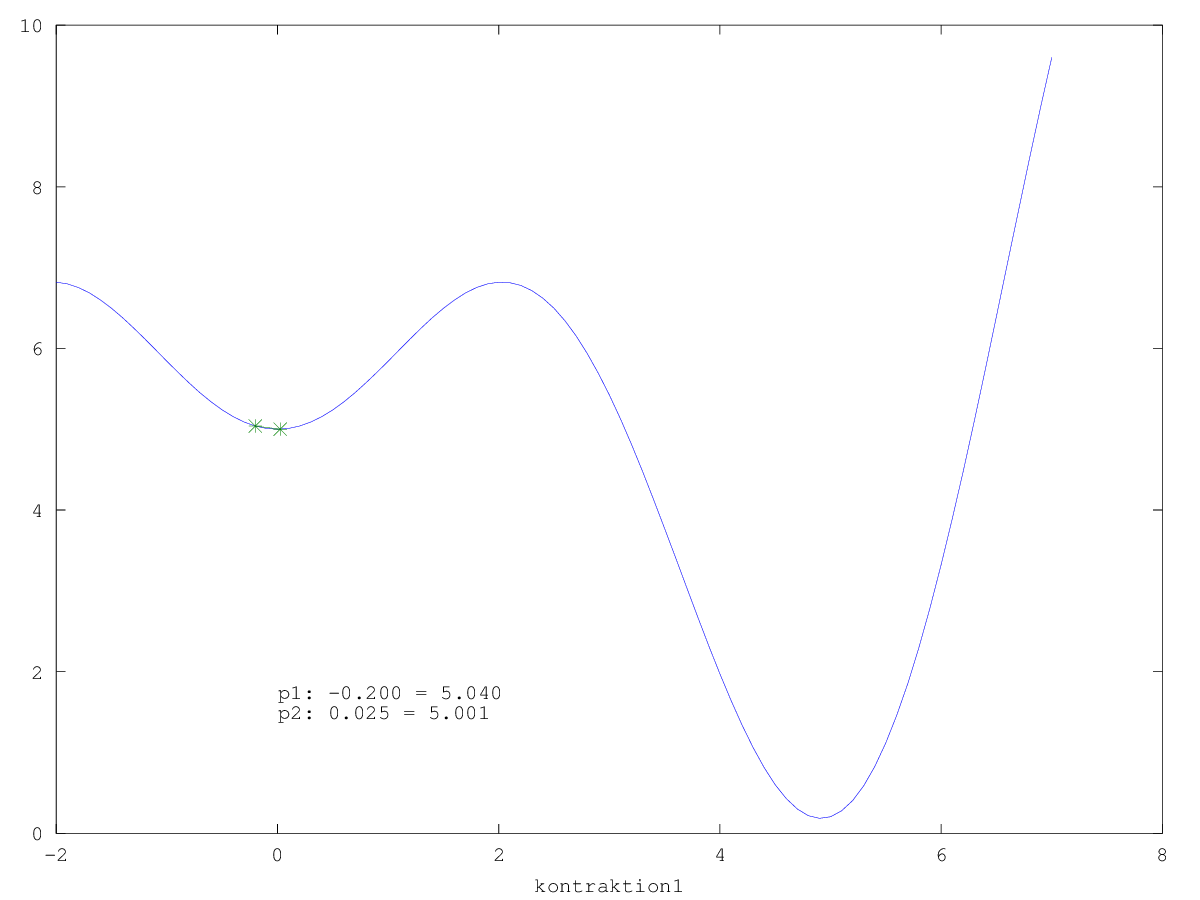
\includegraphics[height=0.75\paperheight]{../bilder/LokMinima/sinx_x006.png}
	\end{center}
\end{frame}
\begin{frame}{Probleme}
	\begin{center}
		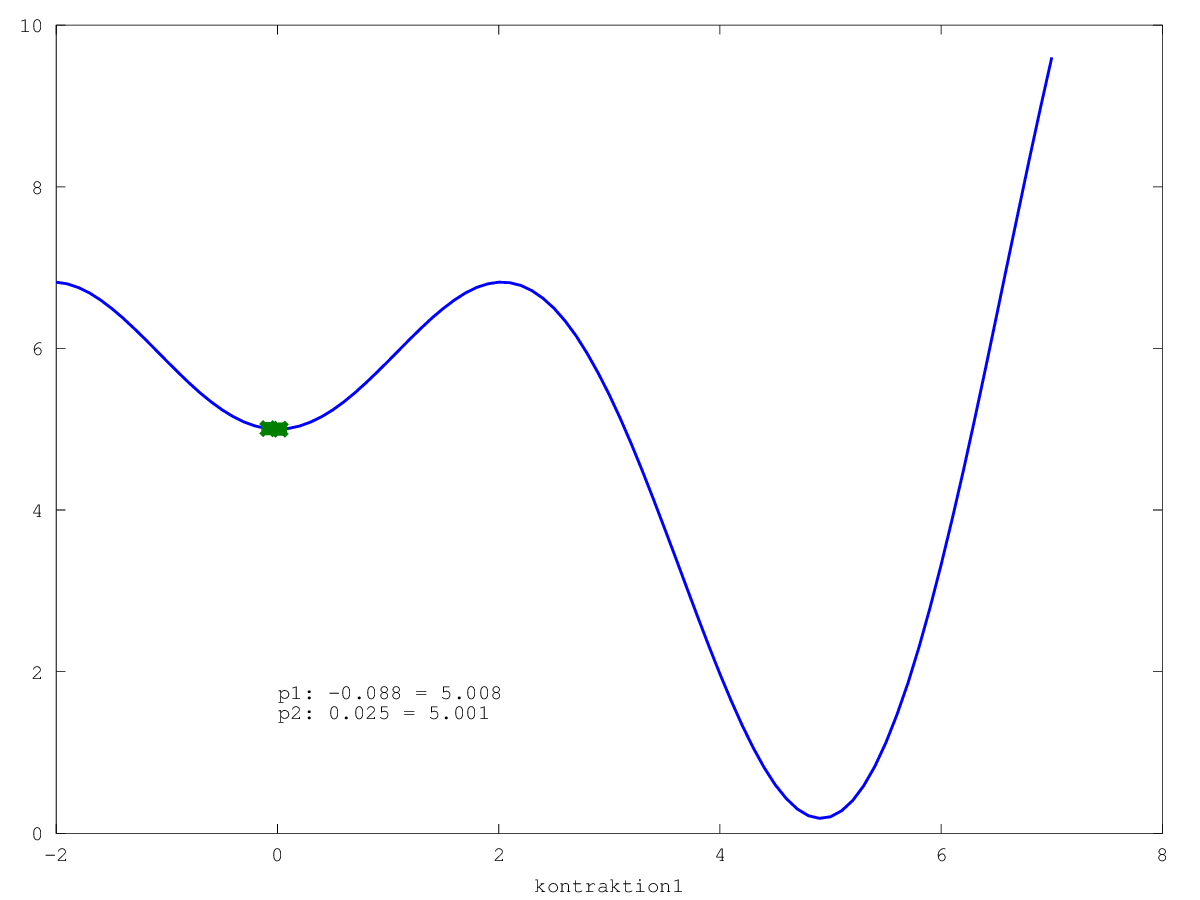
\includegraphics[height=0.75\paperheight]{../bilder/LokMinima/sinx_x007.png}
	\end{center}
\end{frame}
\begin{frame}{Probleme}
	\begin{center}
		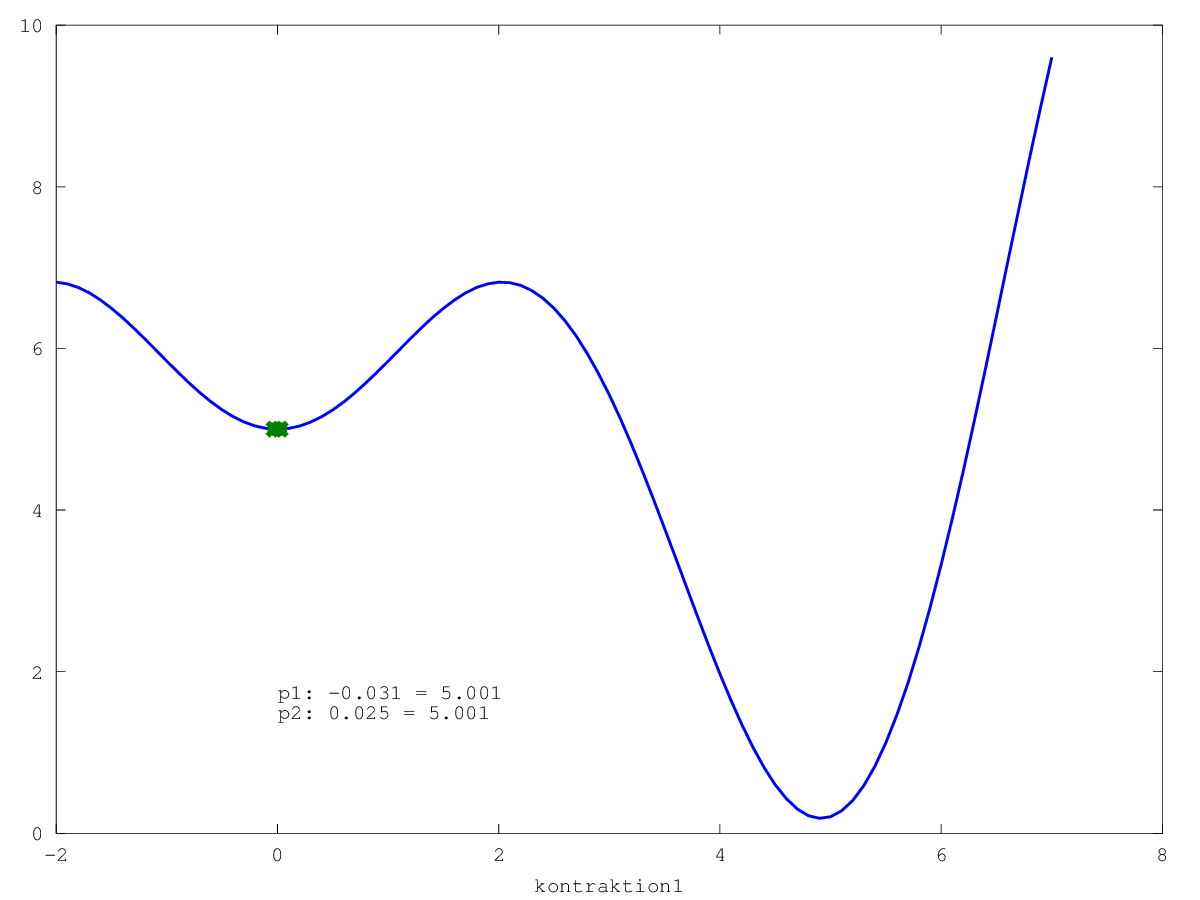
\includegraphics[height=0.75\paperheight]{../bilder/LokMinima/sinx_x008.png}
	\end{center}
\end{frame}
\begin{frame}{Probleme}
	\begin{center}
		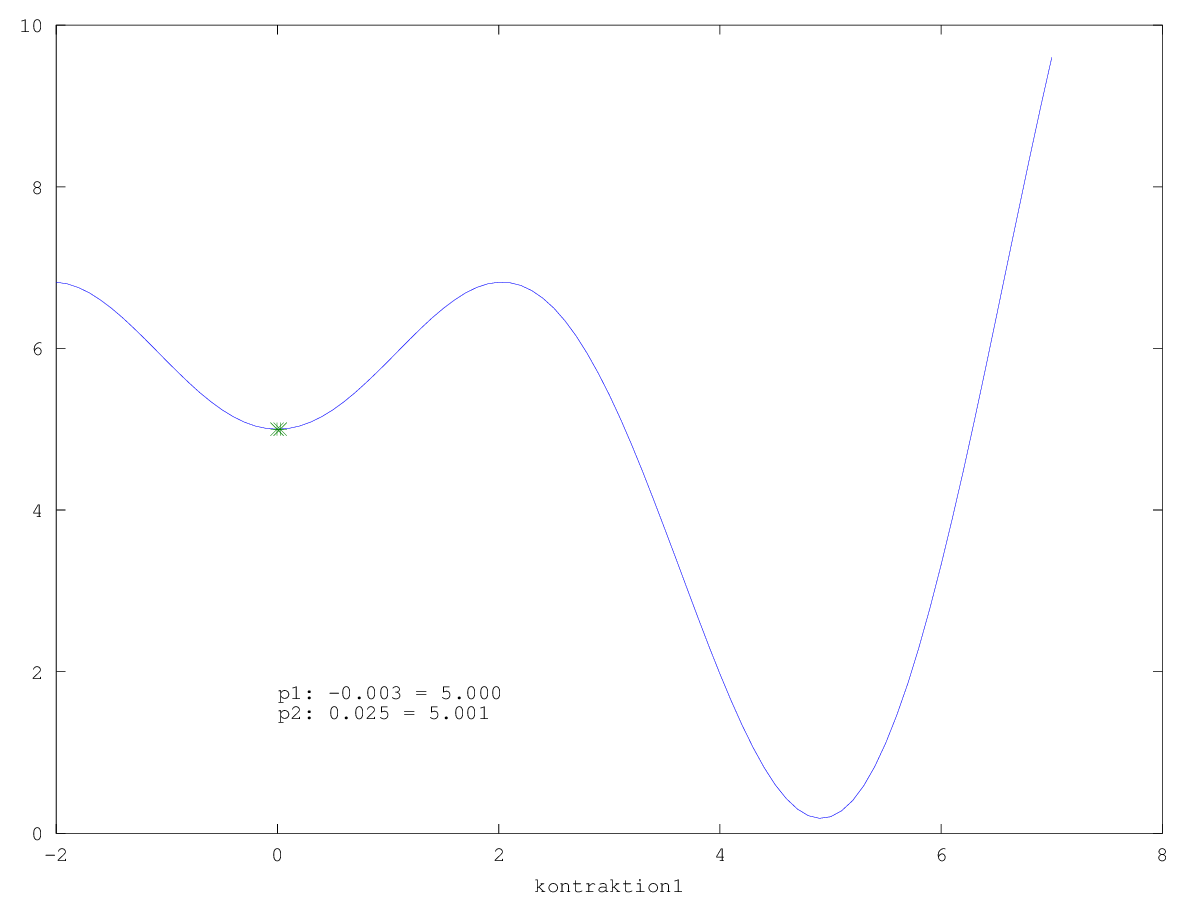
\includegraphics[height=0.75\paperheight]{../bilder/LokMinima/sinx_x009.png}
	\end{center}
\end{frame}
\begin{frame}{Probleme}
	\begin{center}
		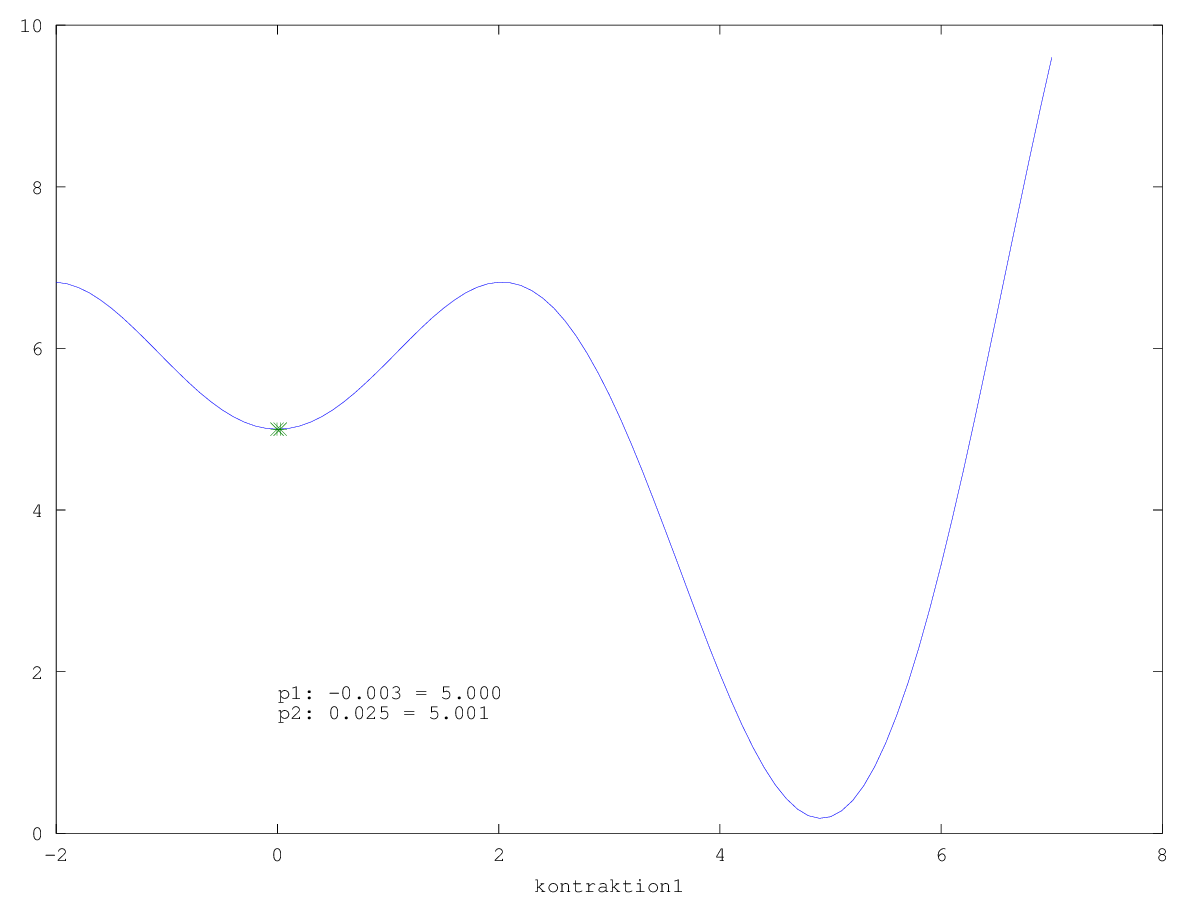
\includegraphics[height=0.75\paperheight]{../bilder/LokMinima/sinx_x009.png}
	\end{center}
\end{frame}

\begin{frame}{Probleme}
\begin{itemize}
\item Lokale Minima
	\begin{itemize}
	\item Neue Startpunkte zufällig wählen
	\end{itemize}
\item An falschem Ort zusammenziehen
	\begin{itemize}
	\item $\beta$ anpassen
	\end{itemize}
\end{itemize}
\end{frame}

% ============================================================================
\section{Parameter} 

\begin{frame}{Parameter}
\begin{itemize}
\item Startpunkte
\begin{itemize}
\item Müssen auf Problem angepasst sein
\item Möglichst orthogonal zueinander
\end{itemize}
\pause \item $\alpha, \beta , \gamma$
\begin{itemize}
\item $\alpha, \gamma$ Schneller ''bewegen`` 
\item $\beta$ Schneller zusammenziehen
\end{itemize}
\end{itemize}
\end{frame}

\begin{frame}{Parameter - Demo}
\end{frame}

\section{Variationen}
\begin{frame}{Variationen}
\begin{itemize}
\item Zusätzlicher Parameter $\sigma$, ersetzt $\beta$ bei Komprimierung
\item Start-Punkte nach zufälliger Zeit neu wählen, wobei der beste Punkt behalten wird
\item Bei Messungen Wahrscheinlichkeit aufgrund des Rauschens miteinbeziehen

\end{itemize}
\end{frame}
\end{document}
